\documentclass[aspectratio=1610]{beamer}
\usetheme[progressbar position=frametitle]{gotham}

\usepackage{ragged2e}
\usepackage{graphicx}
\usepackage{subcaption}
% \usepackage{chngcntr}
\usepackage{enumitem}
\apptocmd{\frame}{}{\justifying}{}
\addtobeamertemplate{block begin}{}{\justifying}
% \setlist[itemize]{noitemsep}



\date{\today}
\title{CSC\_5RO08\_TA, MBSE et Système de Systèmes}
\subtitle{Presentation Projet - Groupe 1}
\author{Daniel FRULANE, Diego PINCER, Gianluca BAGHINO,\\Guilherme NUNES TROFINO et Natalia GALLEGO}
\institute{ENSTA Paris}


\setbeamertemplate{footline}[frame number]
\setbeamercolor{block body}{bg=gray!15, fg=black}
\gothamset{sectiontocframe default=off}
\gothamset{subsectiontocframe default=off}
\titlegraphic{
    \vfill
    \hspace{7.35cm}
    
\includegraphics[width=1cm]{images/800px-Logo_ENSTA_Paris.png}
    \vfill
}




\begin{document}
    \maketitle


    \section{Introduction}
    \begin{frame}{Introduction}
        \tableofcontents
    \end{frame}


    \section*{Previous Work}
    \begin{frame}{Previous Work}
        \begin{figure}[H]
            \centering
            \begin{subfigure}[b]{0.475\textwidth}
                \centering
                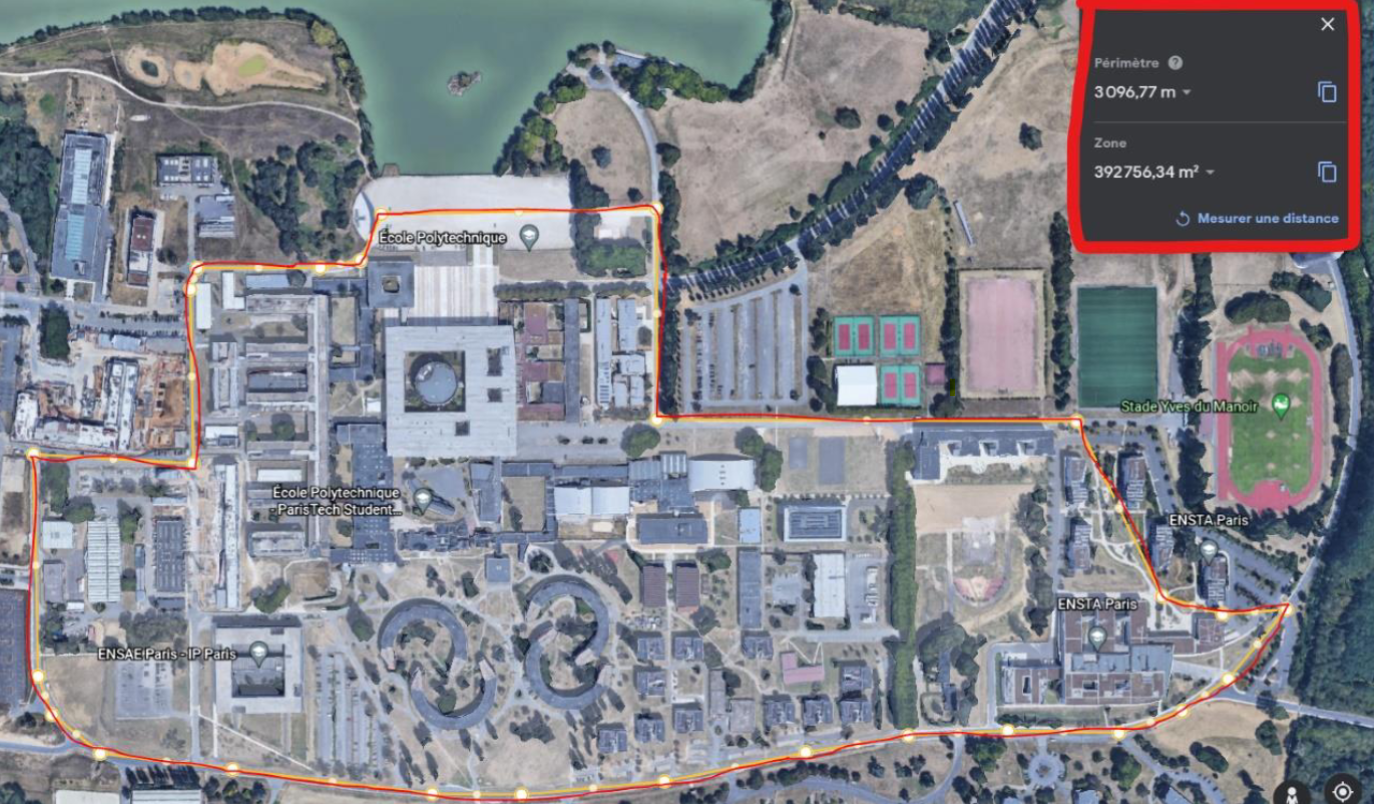
\includegraphics[height=3.75cm]{./images/EX0/CSC_5RO08_TA_path_2.png}
                  \caption{Parcours d'Inspection}
            \end{subfigure}\hfill
            \begin{subfigure}[b]{0.475\textwidth}
                \centering
                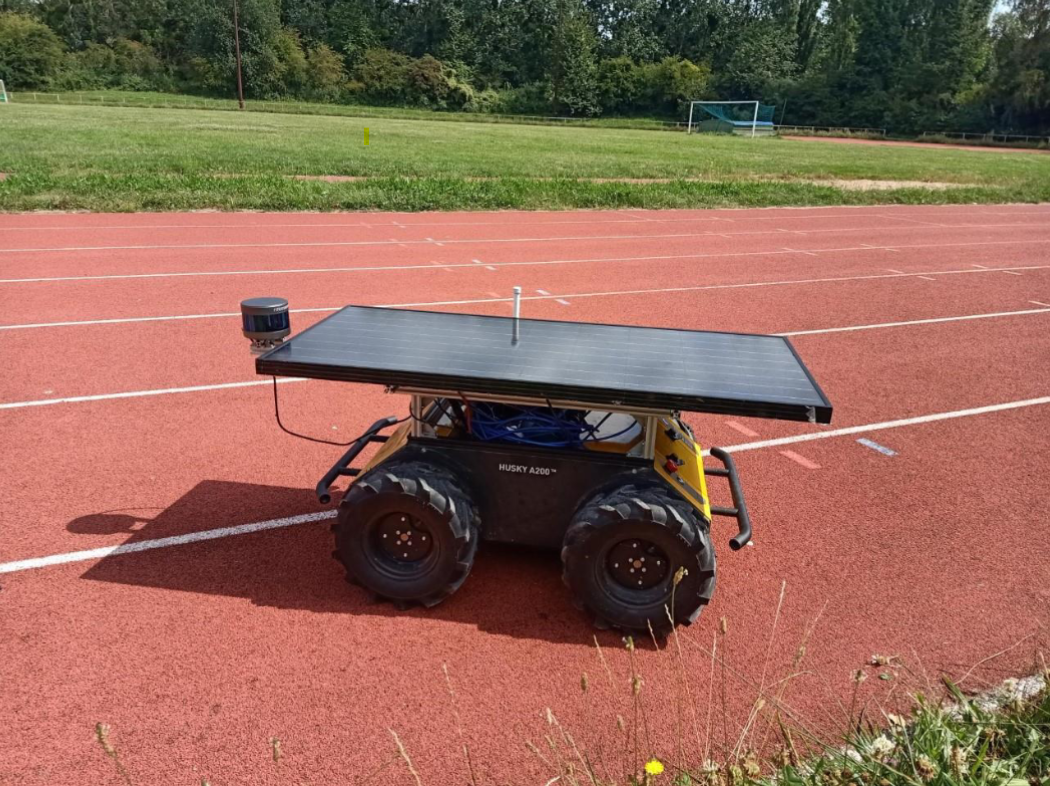
\includegraphics[height=3.75cm]{./images/EX0/CSC_5RO08_TA_robis.png}
                \caption{Robot Robis}
            \end{subfigure}
            \caption{Activité développée en classe}
        \end{figure}
    \end{frame}


    \section{Exercice 1}
    \subsection{Context}
    \begin{frame}{Context}
        \begin{figure}[H]
            \centering
            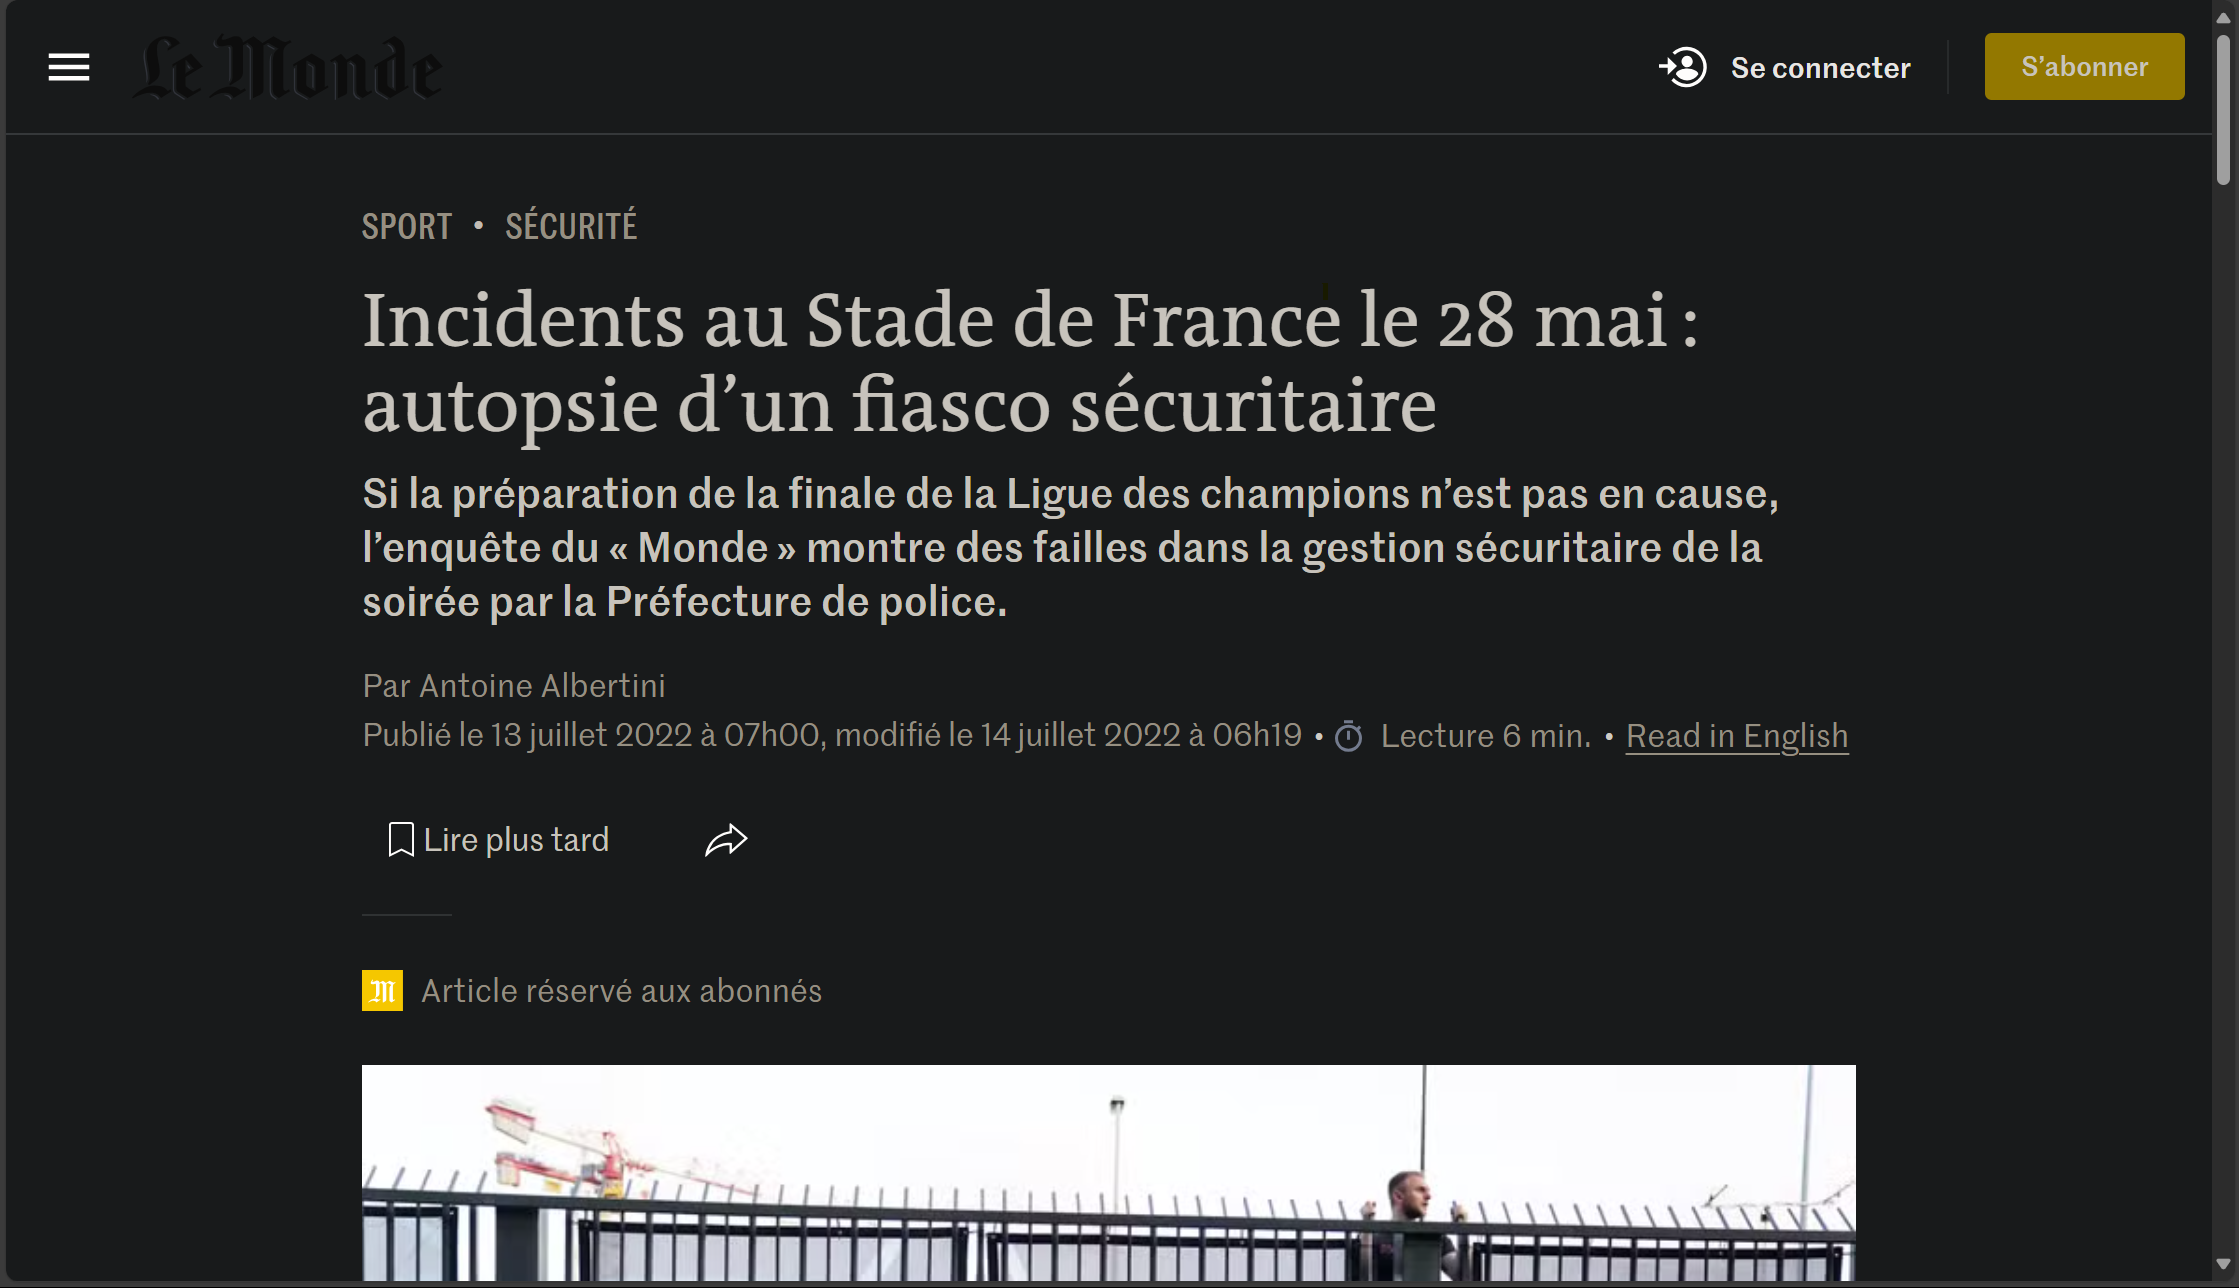
\includegraphics[height=6.5cm]{./images/EX1/CSC_5RO08_TA_EX1_news.png}
            \caption{Finale de la Ligue des Champions 2022}
        \end{figure}
    \end{frame}


    \subsection{Stakeholders}
    \begin{frame}{Exercice 1, Stakeholders}
        Parties prenantes impliquées dans la \textbf{billetterie}, le \textbf{transport} et les \textbf{contrôles d'accès}:
        \begin{itemize}[noitemsep]
            \item UEFA
            \item FFF, Fédération Française de Football
            \item SF, Stade de France
            \item TM, TicketMaster
            \item RATP \& SNCF
            \item ADP, Aéroports de Paris
            \item Sécurité Privée \& Personnel
            \item Clubs Participants, Liverpool \& Real Madrid
        \end{itemize}
    \end{frame}
    \begin{frame}{Exercice 1, Stakeholders}
        Parties prenantes impliquées dans la gestion de \textbf{l'ordre public} et de la \textbf{sécurité}:
        \begin{itemize}[noitemsep]
            \item MI, Ministère de l'Intérieur
            \item PPP, Préfecture de Police de Paris
            \item GN, Gendarmerie Nationale
            \item PN, Police Nationale \& CRS
            \item Pompiers de Paris
            \item SAMU
            \item MSDP, Mairie de Saint-Denis et de Paris
            \item ODDH, Organisations de Défense des Droits Humains
        \end{itemize}
    \end{frame}

    \subsection{Diagrammes}
    \begin{frame}{Exercice 1, Operational Entity BreakDown}
        \begin{figure}[H]
            \centering
            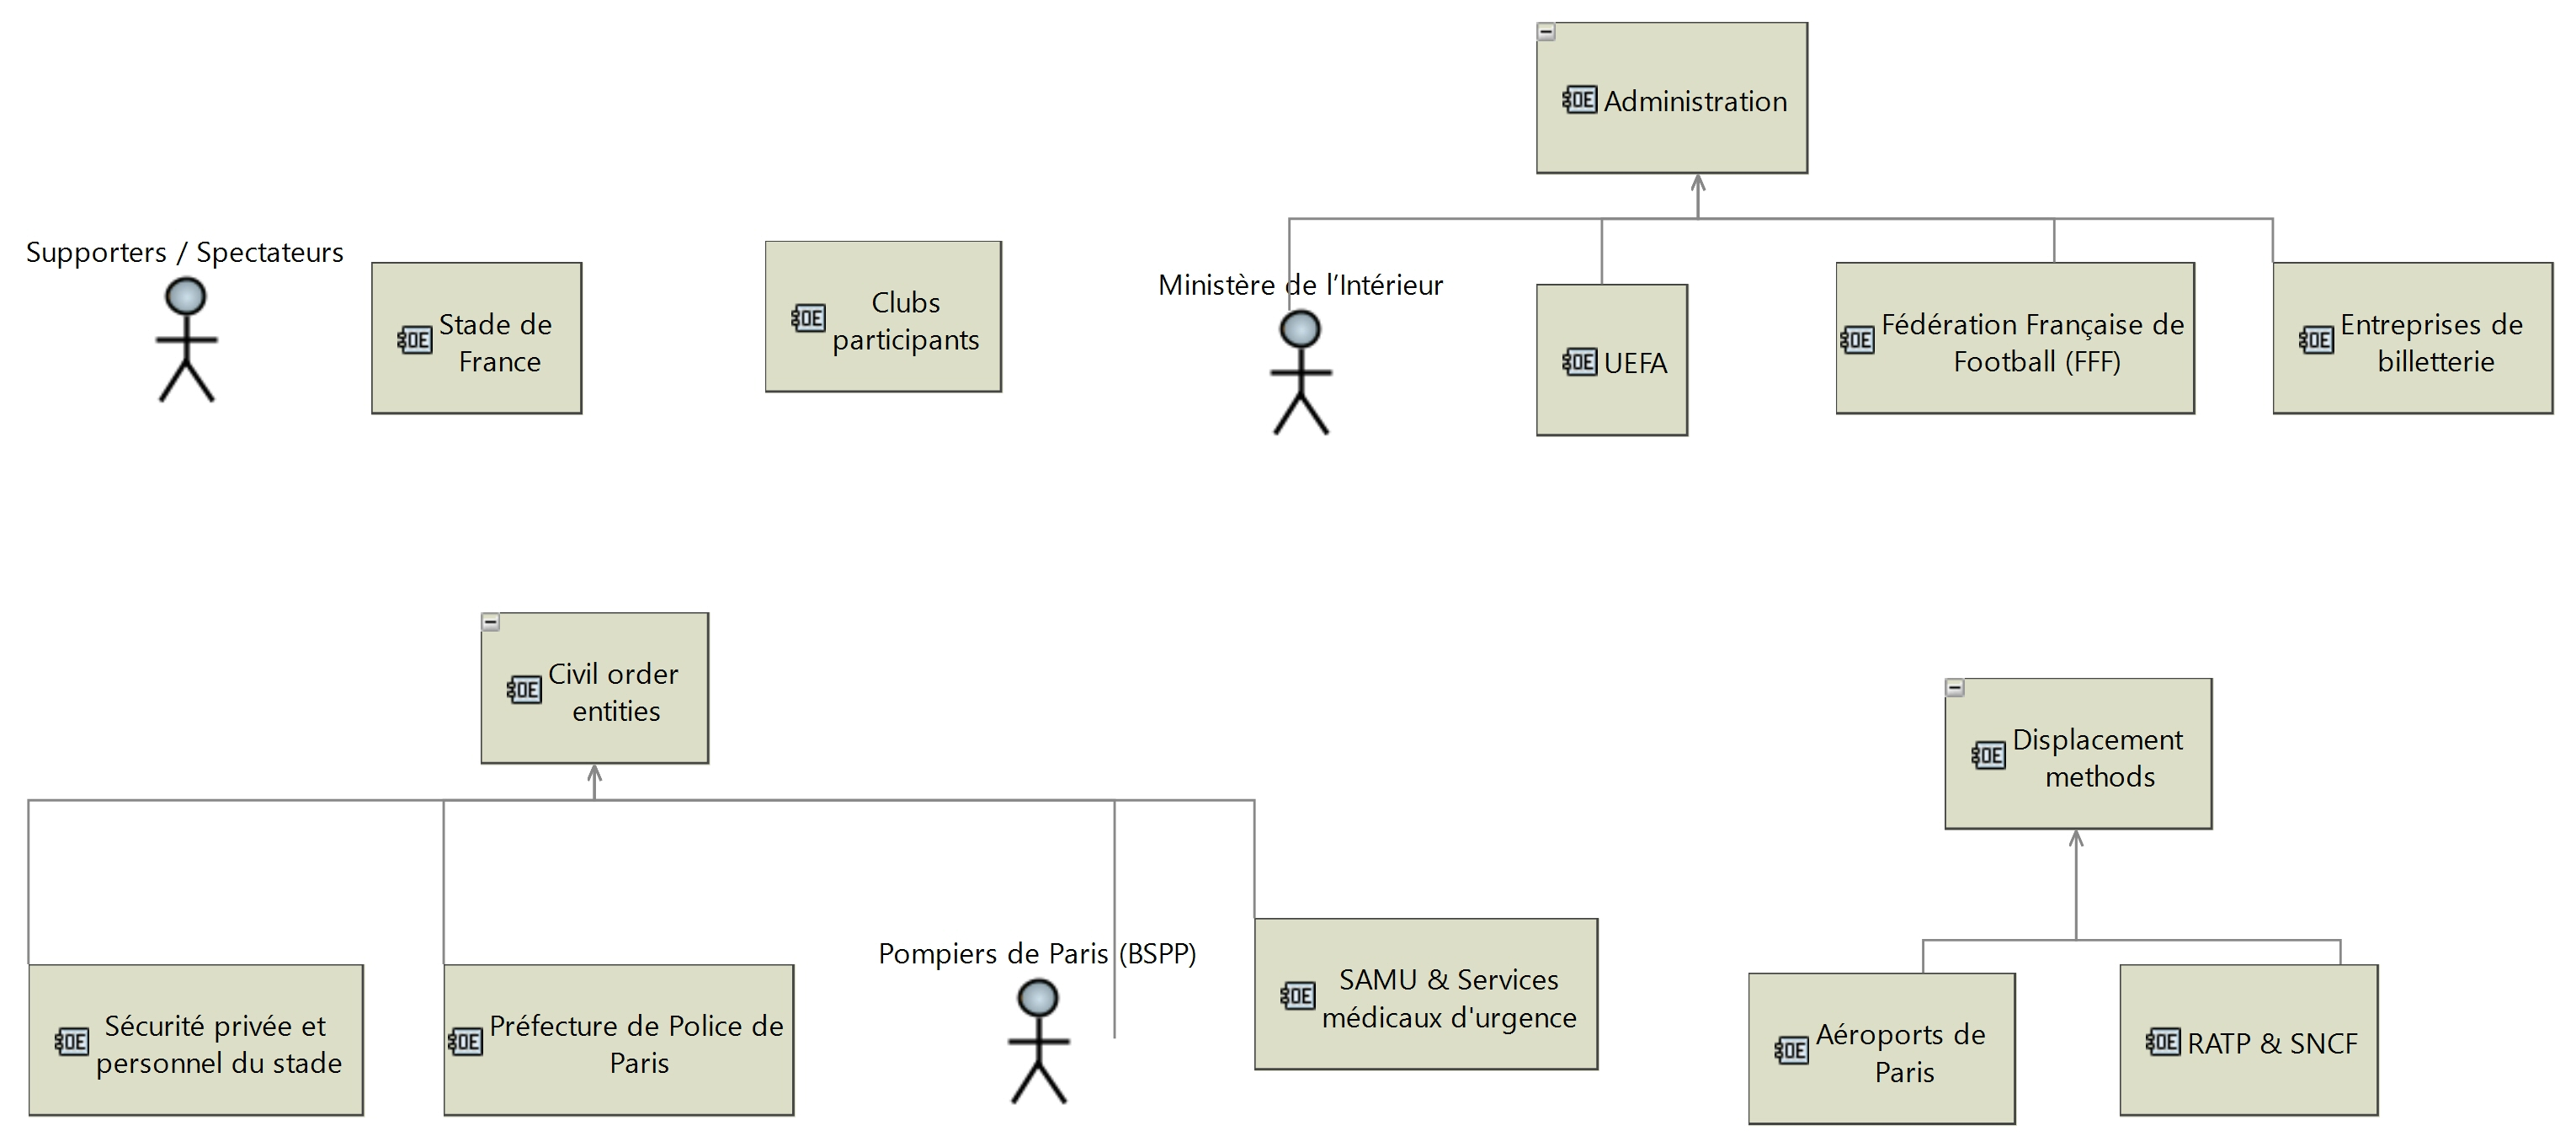
\includegraphics[width=\textwidth, height=6.75cm, keepaspectratio]{./images/EX1/CSC_5RO08_TA_EX1_OEBD.jpg}
            % \caption{Operational Entity BreakDown}
        \end{figure}
    \end{frame}
    \begin{frame}{Exercice 1, Matrice d'Influence et d'Intérêt}
        \begin{table}[]
            \begin{tabular}{llll}
            \hline
            \multicolumn{1}{c}{Partie Prenante}             & \multicolumn{1}{c}{Influence} & \multicolumn{1}{c}{Intérêt} & \multicolumn{1}{c}{Positionnement}  \\ \hline\hline
                        UEFA                                & \textbf{Élevée}               & \textbf{Élevé}              & Décisions stratégiques              \\
                        FFF                                 & \textbf{Élevée}               & \textbf{Élevé}              & Gestion nationale                   \\
                        Stade de France                     & \textbf{Élevée}               & \textbf{Élevé}              & Infrastructure et logistique        \\
                        Ministère de l'Intérieur            & \textbf{Élevée}               & Moyen                       & Sécurité et ordre public            \\
                        Préfecture de Police de Paris       & \textbf{Élevée}               & \textbf{Élevé}              & Coordination sécuritaire            \\
                        Gendarmerie Nationale               & Moyenne                       & \textbf{Élevé}              & Soutien sécuritaire                 \\
                        TicketMaster                        & Moyenne                       & \textbf{Élevé}              & Prévention de la fraude             \\
                        RATP/SNCF                           & Moyenne                       & \textbf{Élevé}              & Flux des spectateurs                \\
                        Aéroports de Paris                  & Moyenne                       & Moyen                       & Connexion visiteurs                 \\
                        Pompiers de Paris                   & Moyenne                       & \textbf{Élevé}              & Sécurité incendie et secours        \\
                        SAMU                                & Moyenne                       & \textbf{Élevé}              & Réponse médicale                    \\
                        Mairie de Saint-Denis et de Paris   & Moyenne                       & Moyen                       & Gestion urbaine                     \\
                        Organisations de Défense des DH     & Faible                        & \textbf{Élevé}              & Protection des droits               \\ \hline
            \end{tabular}
        \end{table}
    \end{frame}
    \begin{frame}{Exercice 1, Component and System Architecture}
        \begin{figure}[H]
            \centering
            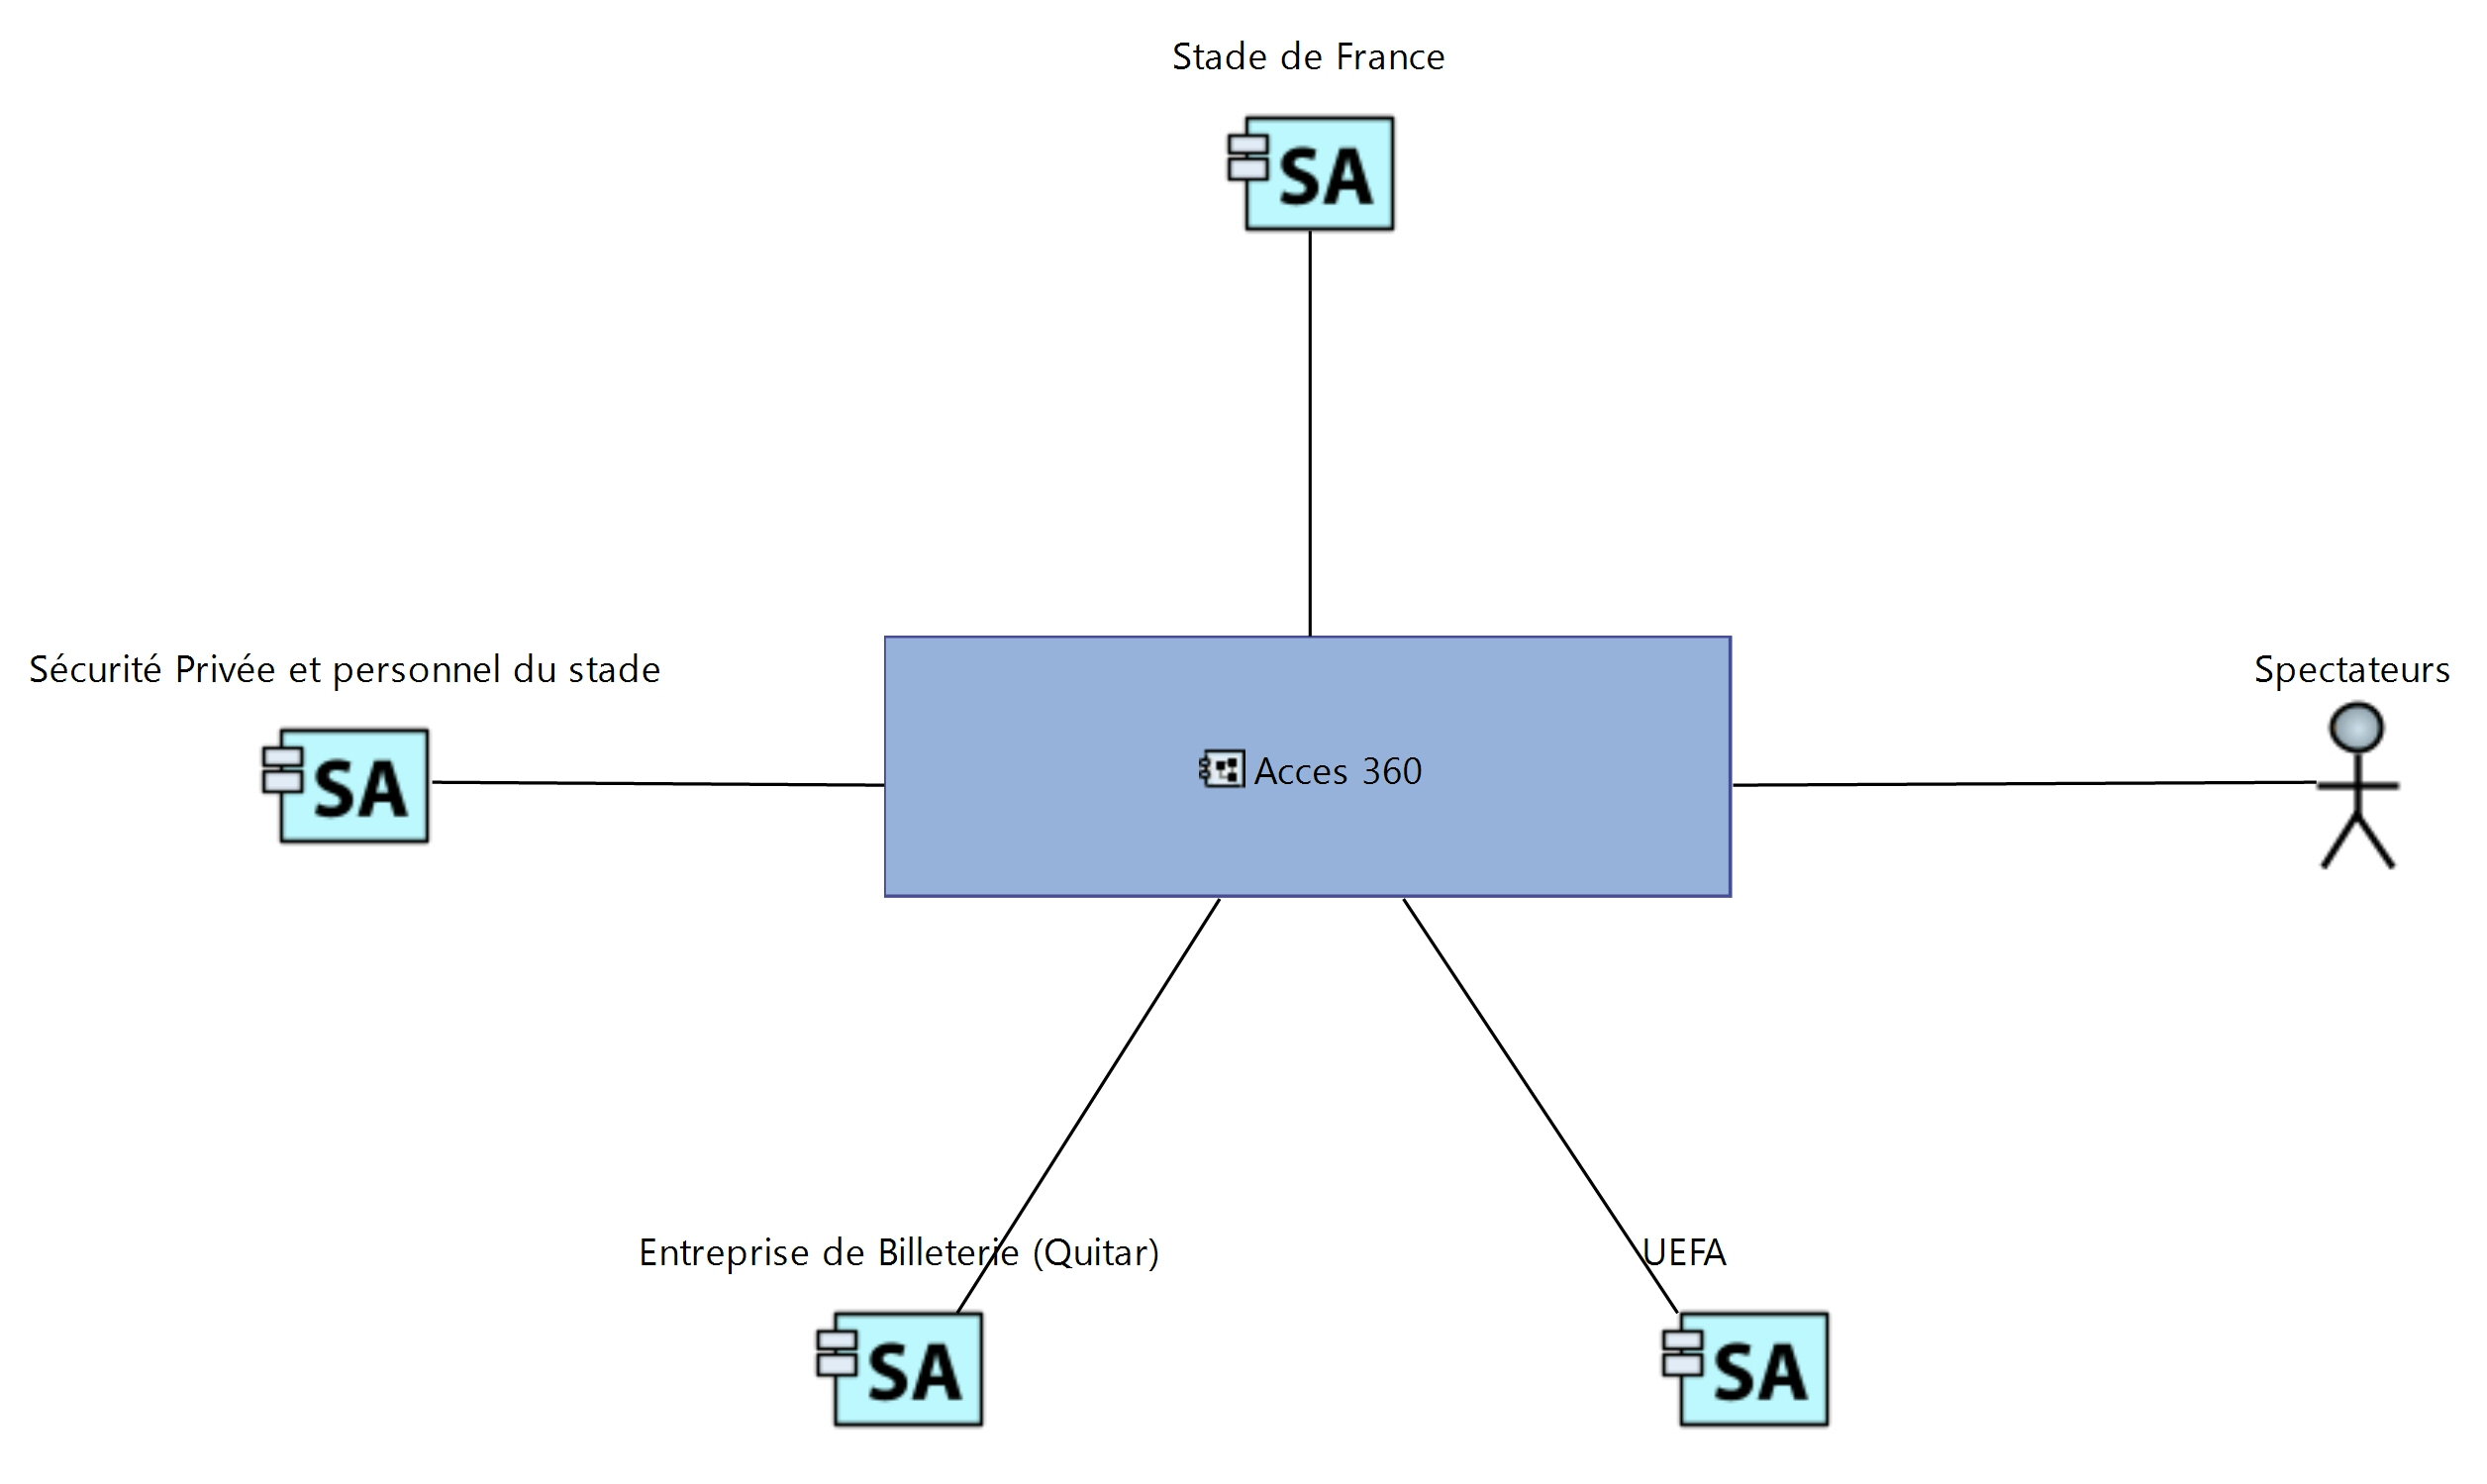
\includegraphics[width=\textwidth, height=6.75cm, keepaspectratio]{./images/EX1/CSC_5RO08_TA_EX1_CSA.jpg}
            % \caption{CSA}
        \end{figure}
    \end{frame}
    \begin{frame}{Exercice 1, Mission and Capabilities Blank}
        \begin{figure}[H]
            \centering
            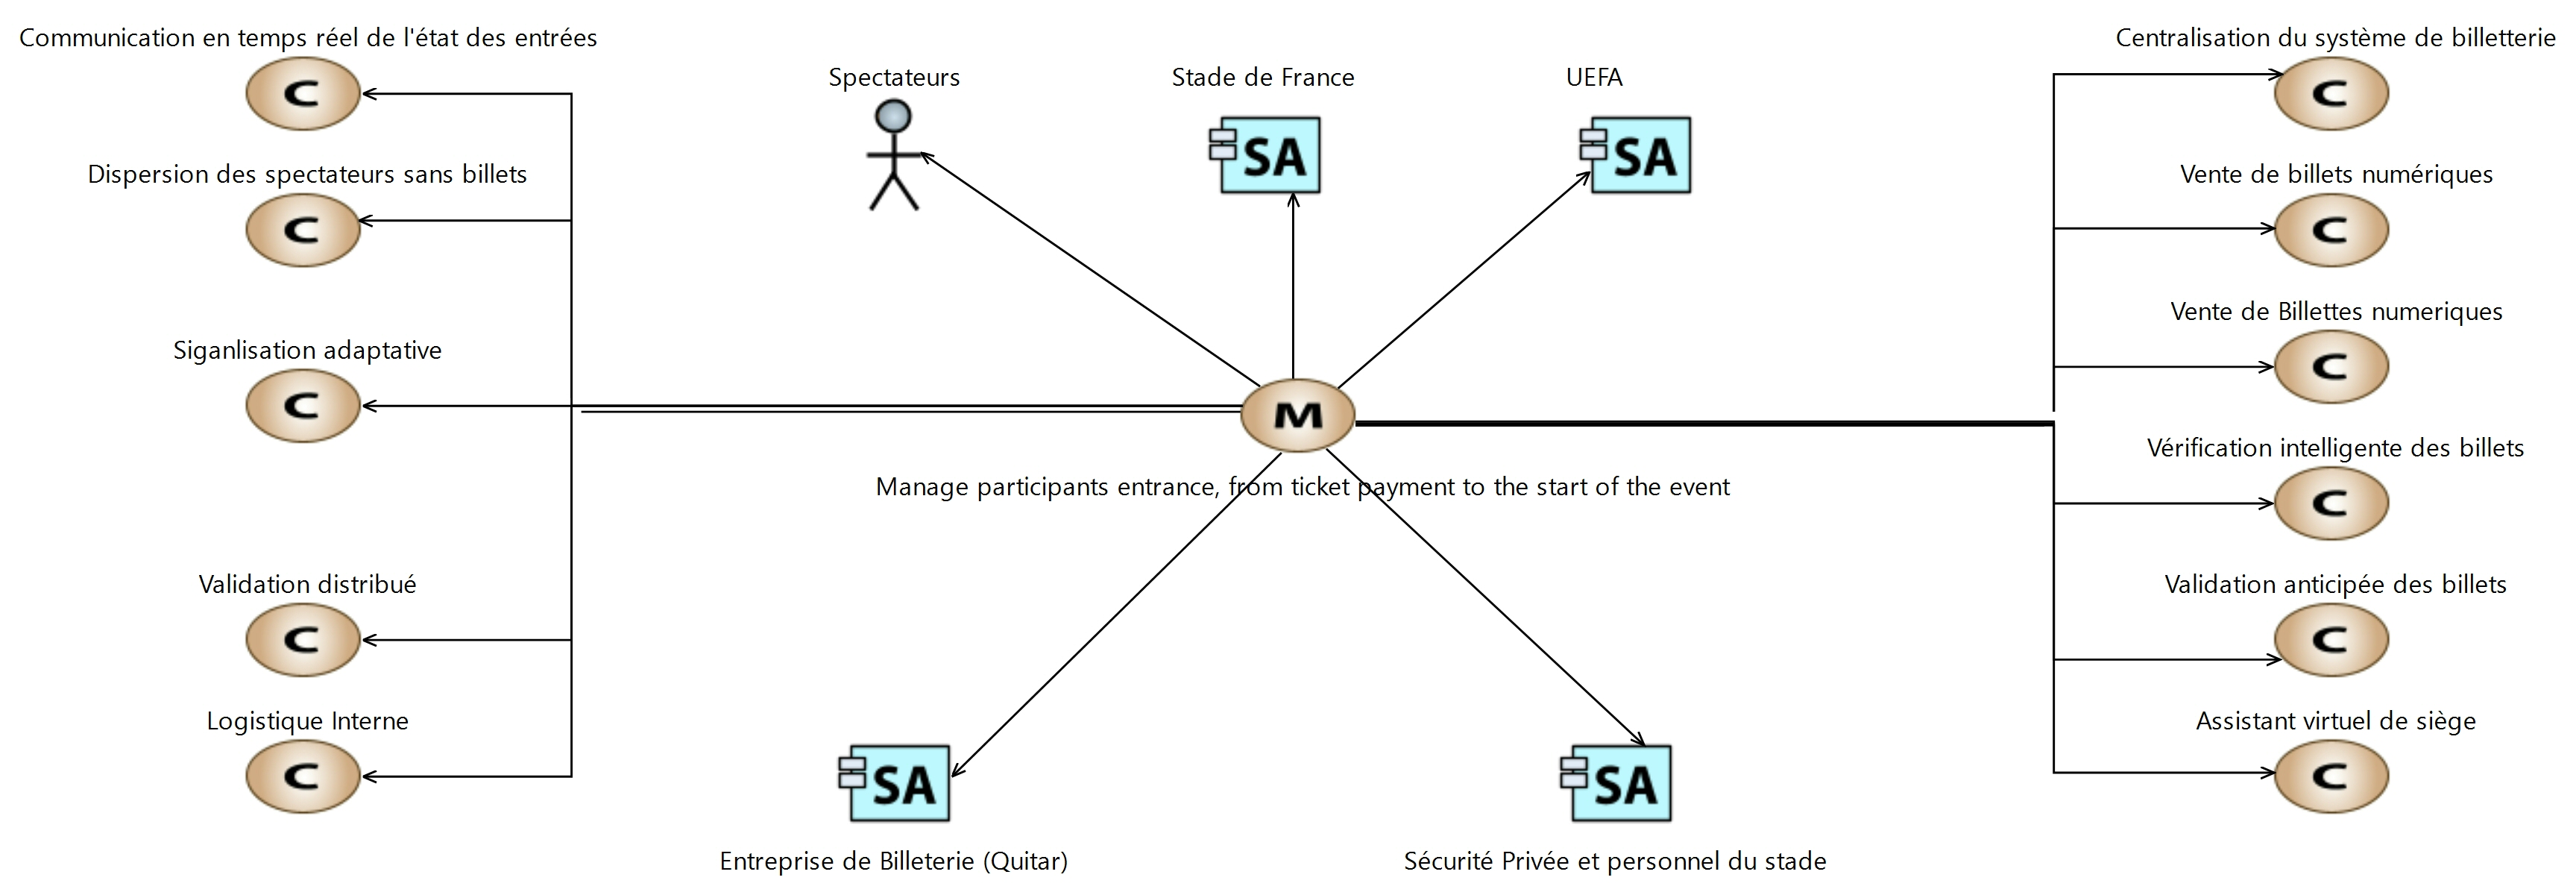
\includegraphics[width=\textwidth, height=6.75cm, keepaspectratio]{./images/EX1/CSC_5RO08_TA_EX1_MCB.jpg}
            % \caption{MCB}
        \end{figure}
    \end{frame}
    \begin{frame}{Exercice 1, Physical Architecture Blank}
        \begin{figure}[H]
            \centering
            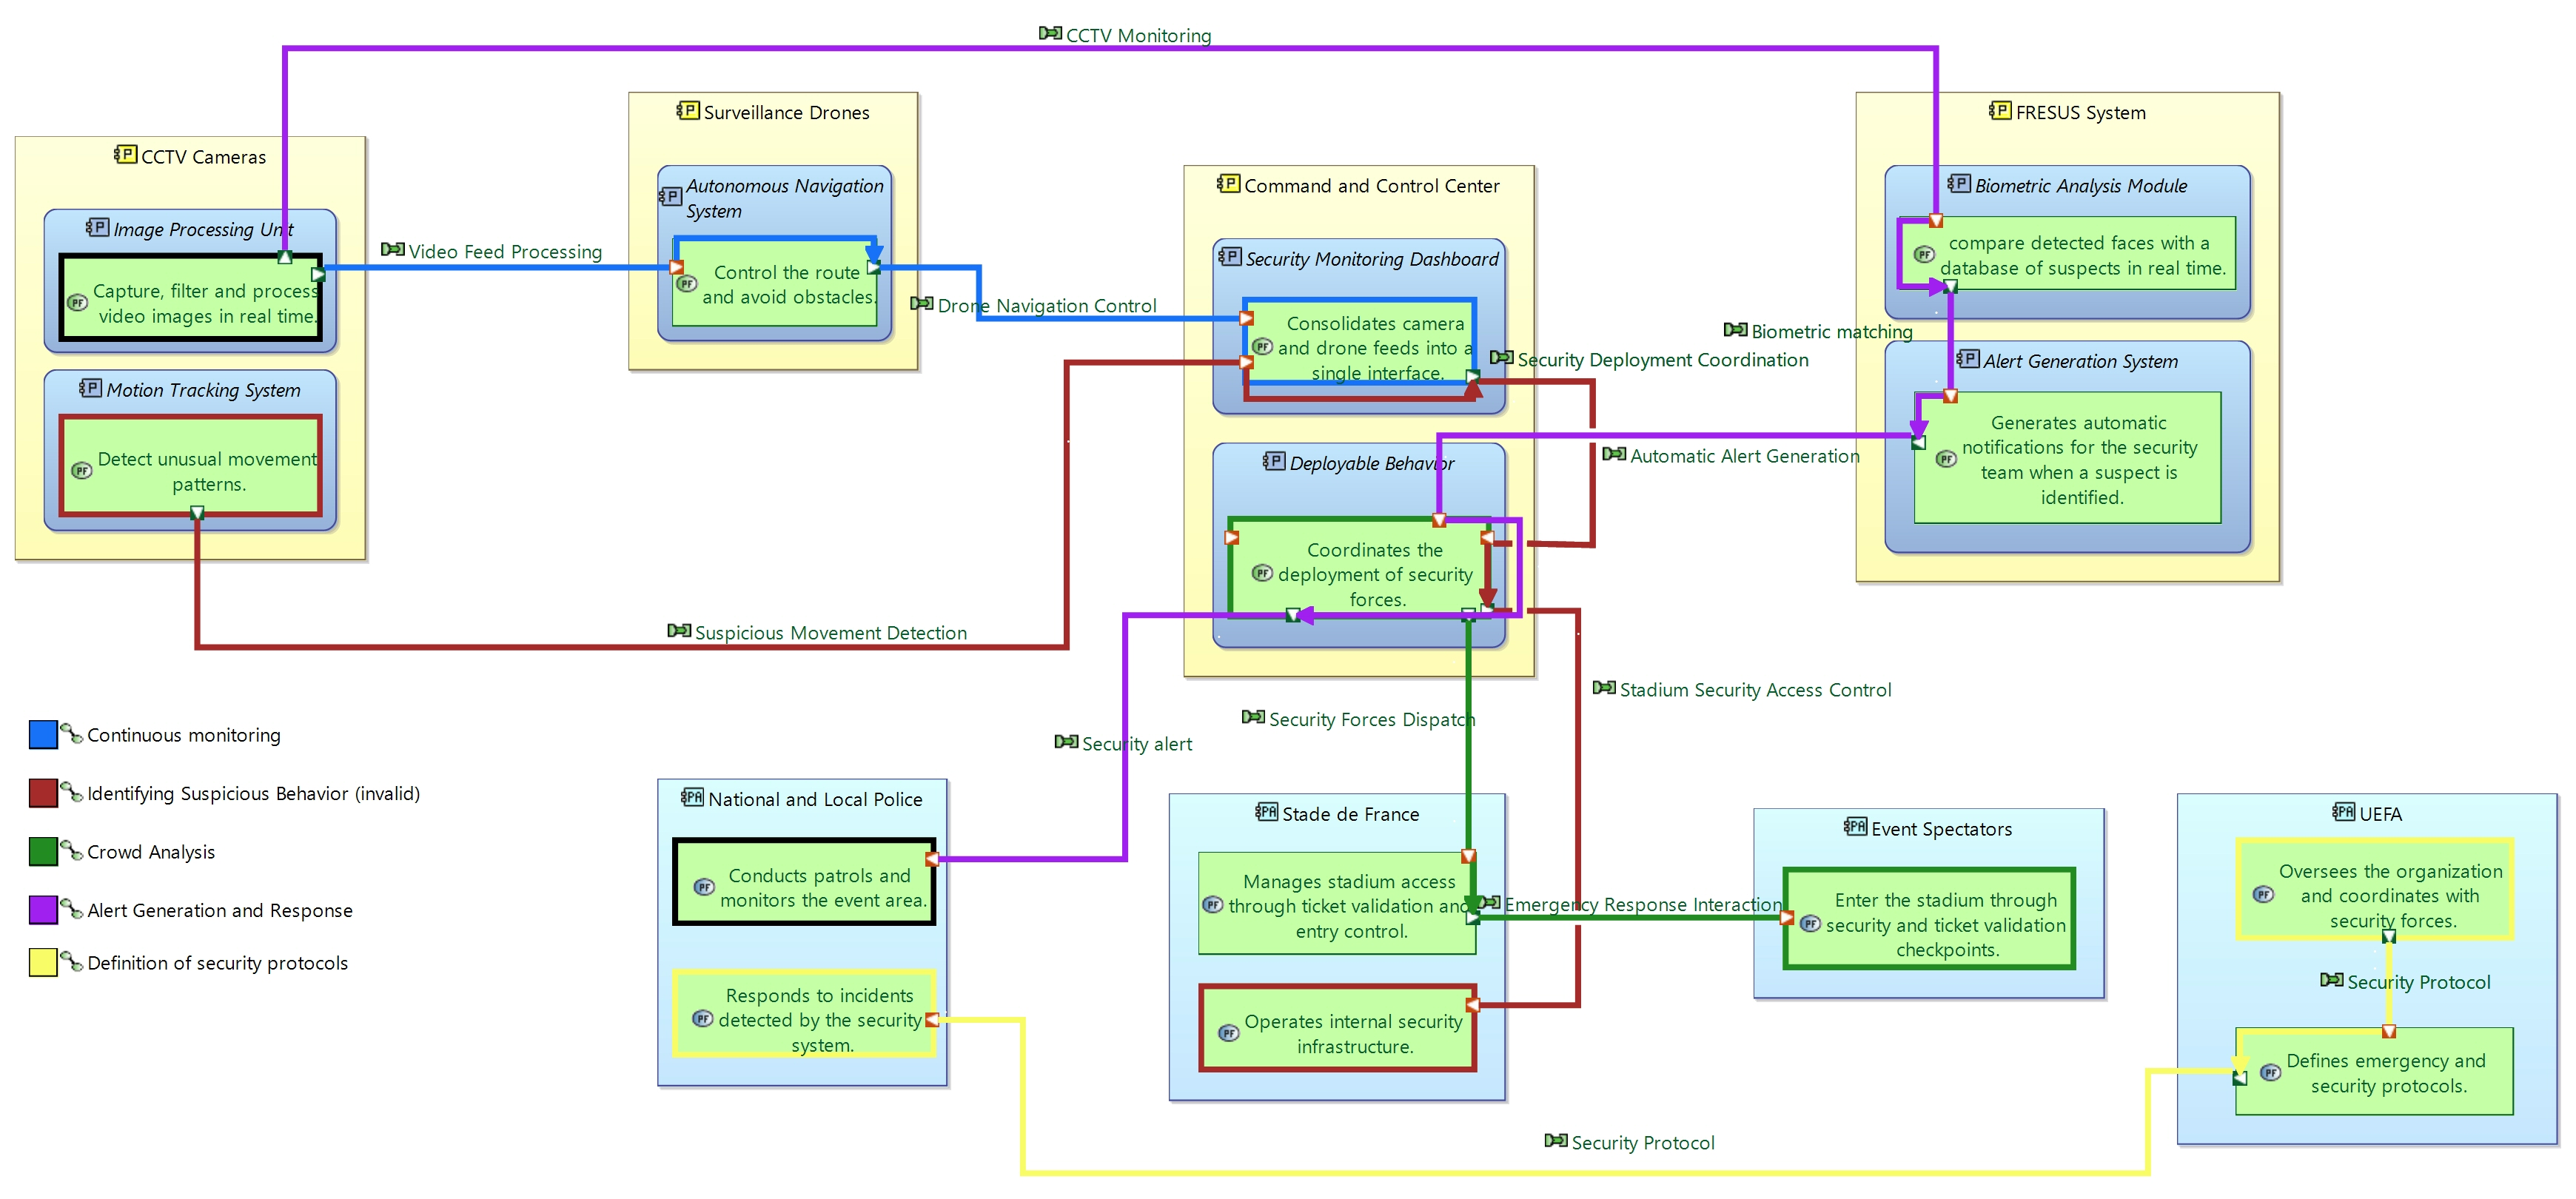
\includegraphics[width=\textwidth, height=6.75cm, keepaspectratio]{./images/EX1/CSC_5RO08_TA_EX1_PAB.jpg}
            % \caption{Physical Architecture Blank}
        \end{figure}
    \end{frame}



    \section{Exercice 2}

    \subsection{Filtres}
    \begin{frame}{Exercice 2, High Performance}
        \begin{figure}[H]
            \centering
            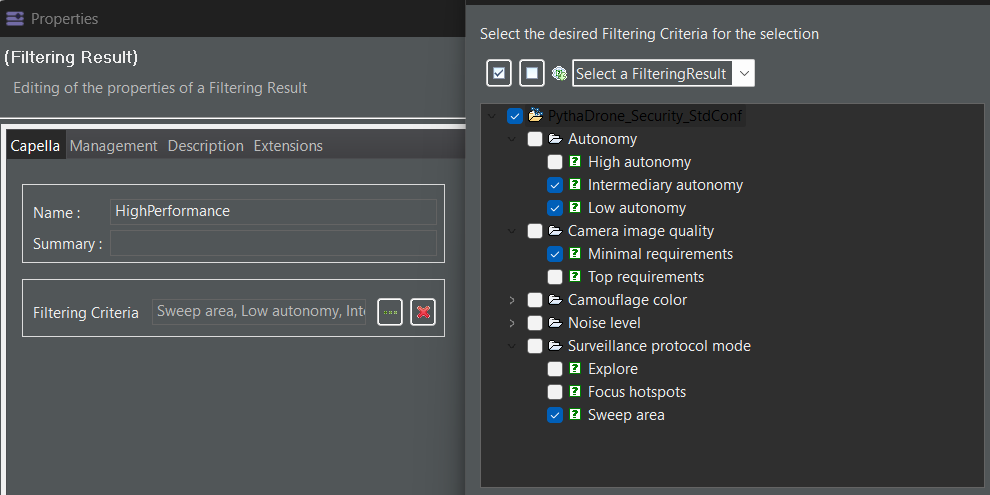
\includegraphics[width=\textwidth, height=6cm, keepaspectratio]{./images/EX2/CSC_5RO08_TA_EX2_Filter_High.png}
            % \caption{}
        \end{figure}
    \end{frame}
    \begin{frame}{Exercice 2, Hybride Performance}
        \begin{figure}[H]
            \centering
            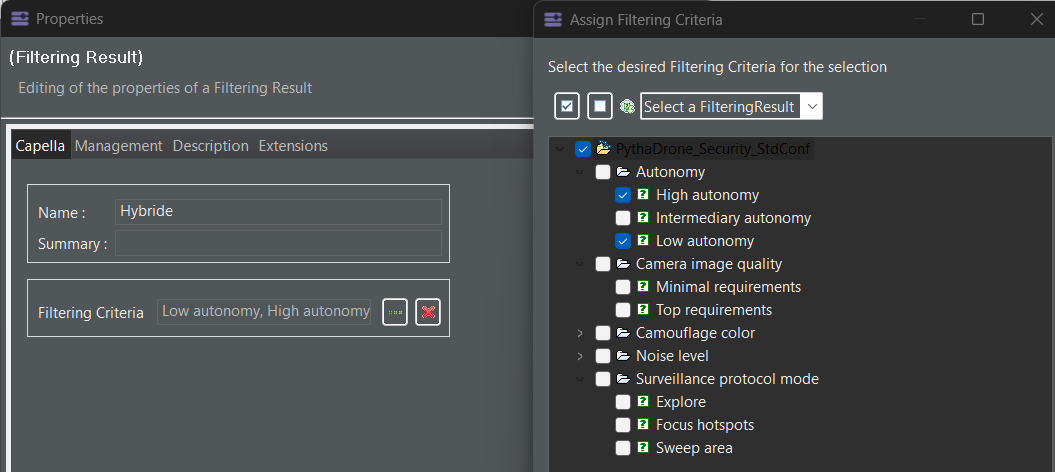
\includegraphics[width=\textwidth, height=6cm, keepaspectratio]{./images/EX2/CSC_5RO08_TA_EX2_Filter_Hybride.png}
            % \caption{}
        \end{figure}
    \end{frame}
    \begin{frame}{Exercice 2, Low Performance}
        \begin{figure}[H]
            \centering
            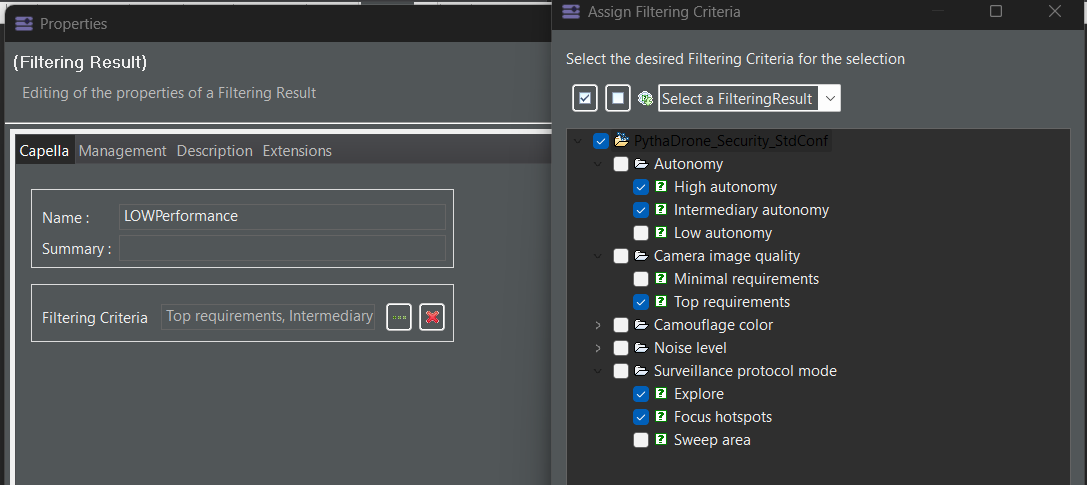
\includegraphics[width=\textwidth, height=6cm, keepaspectratio]{./images/EX2/CSC_5RO08_TA_EX2_Filter_Low.png}
            % \caption{}
        \end{figure}
    \end{frame}

    \subsection{MCB}
    \begin{frame}{Exercice 2, MCB}
        \begin{figure}[H]
            \centering
            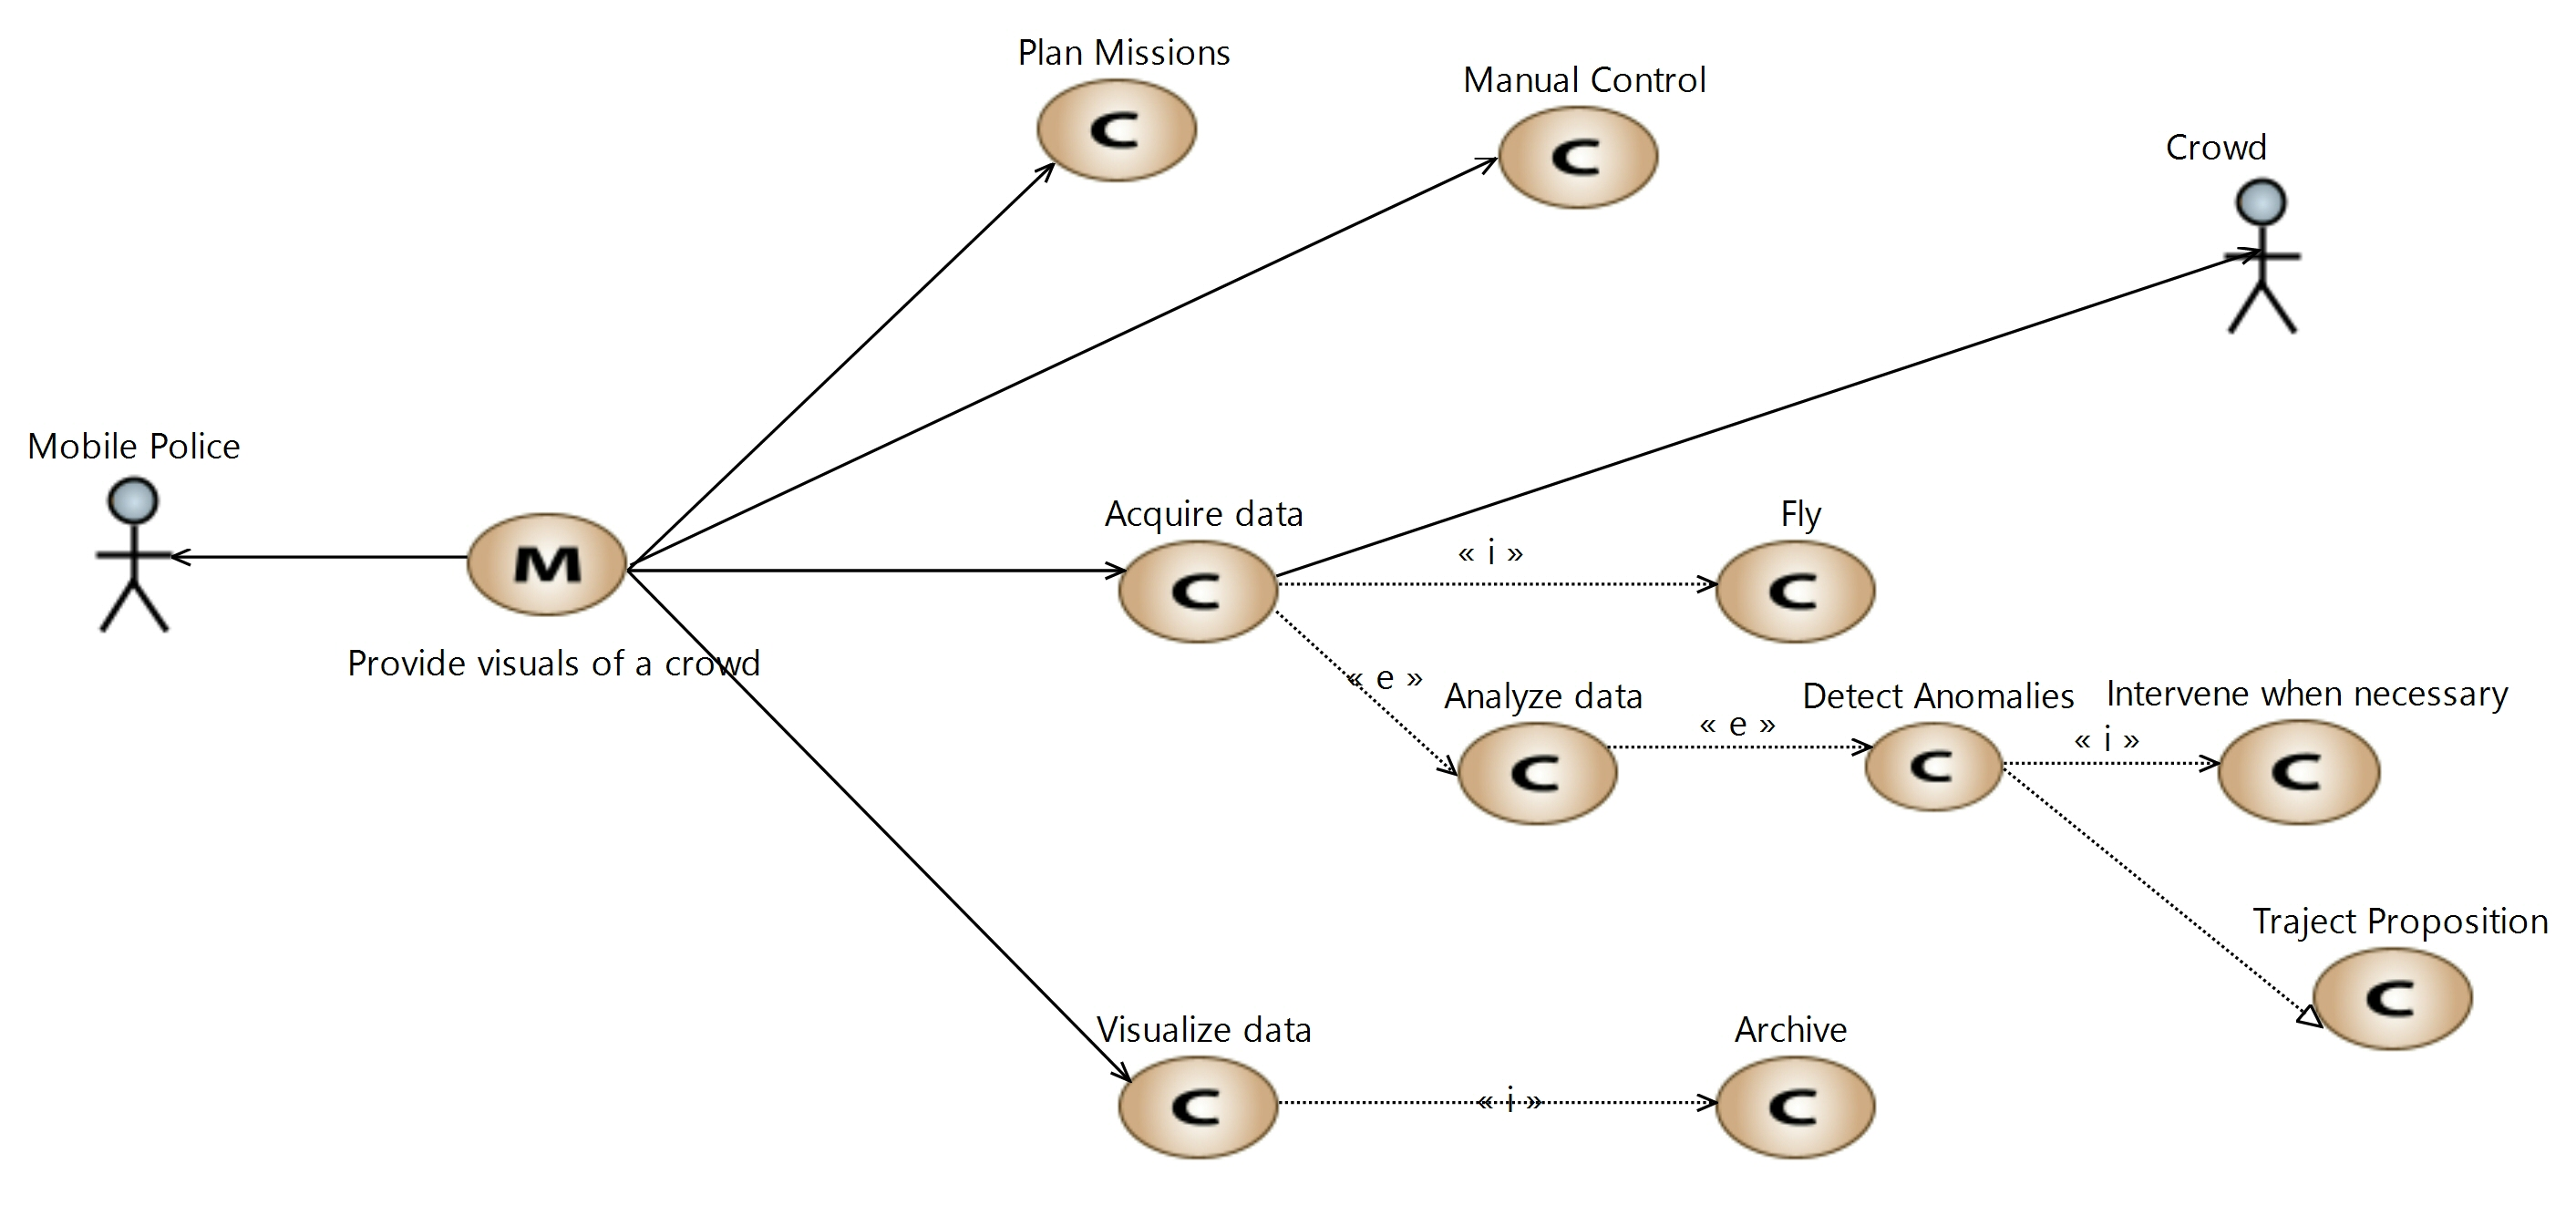
\includegraphics[width=\textwidth, height=6.75cm, keepaspectratio]{./images/EX2/CSC_5RO08_TA_EX2_MCB_Orginal.jpg}
            % \caption{}
        \end{figure}
    \end{frame}
    \begin{frame}{Exercice 2, MCB - High Performance}
        \begin{figure}[H]
            \centering
            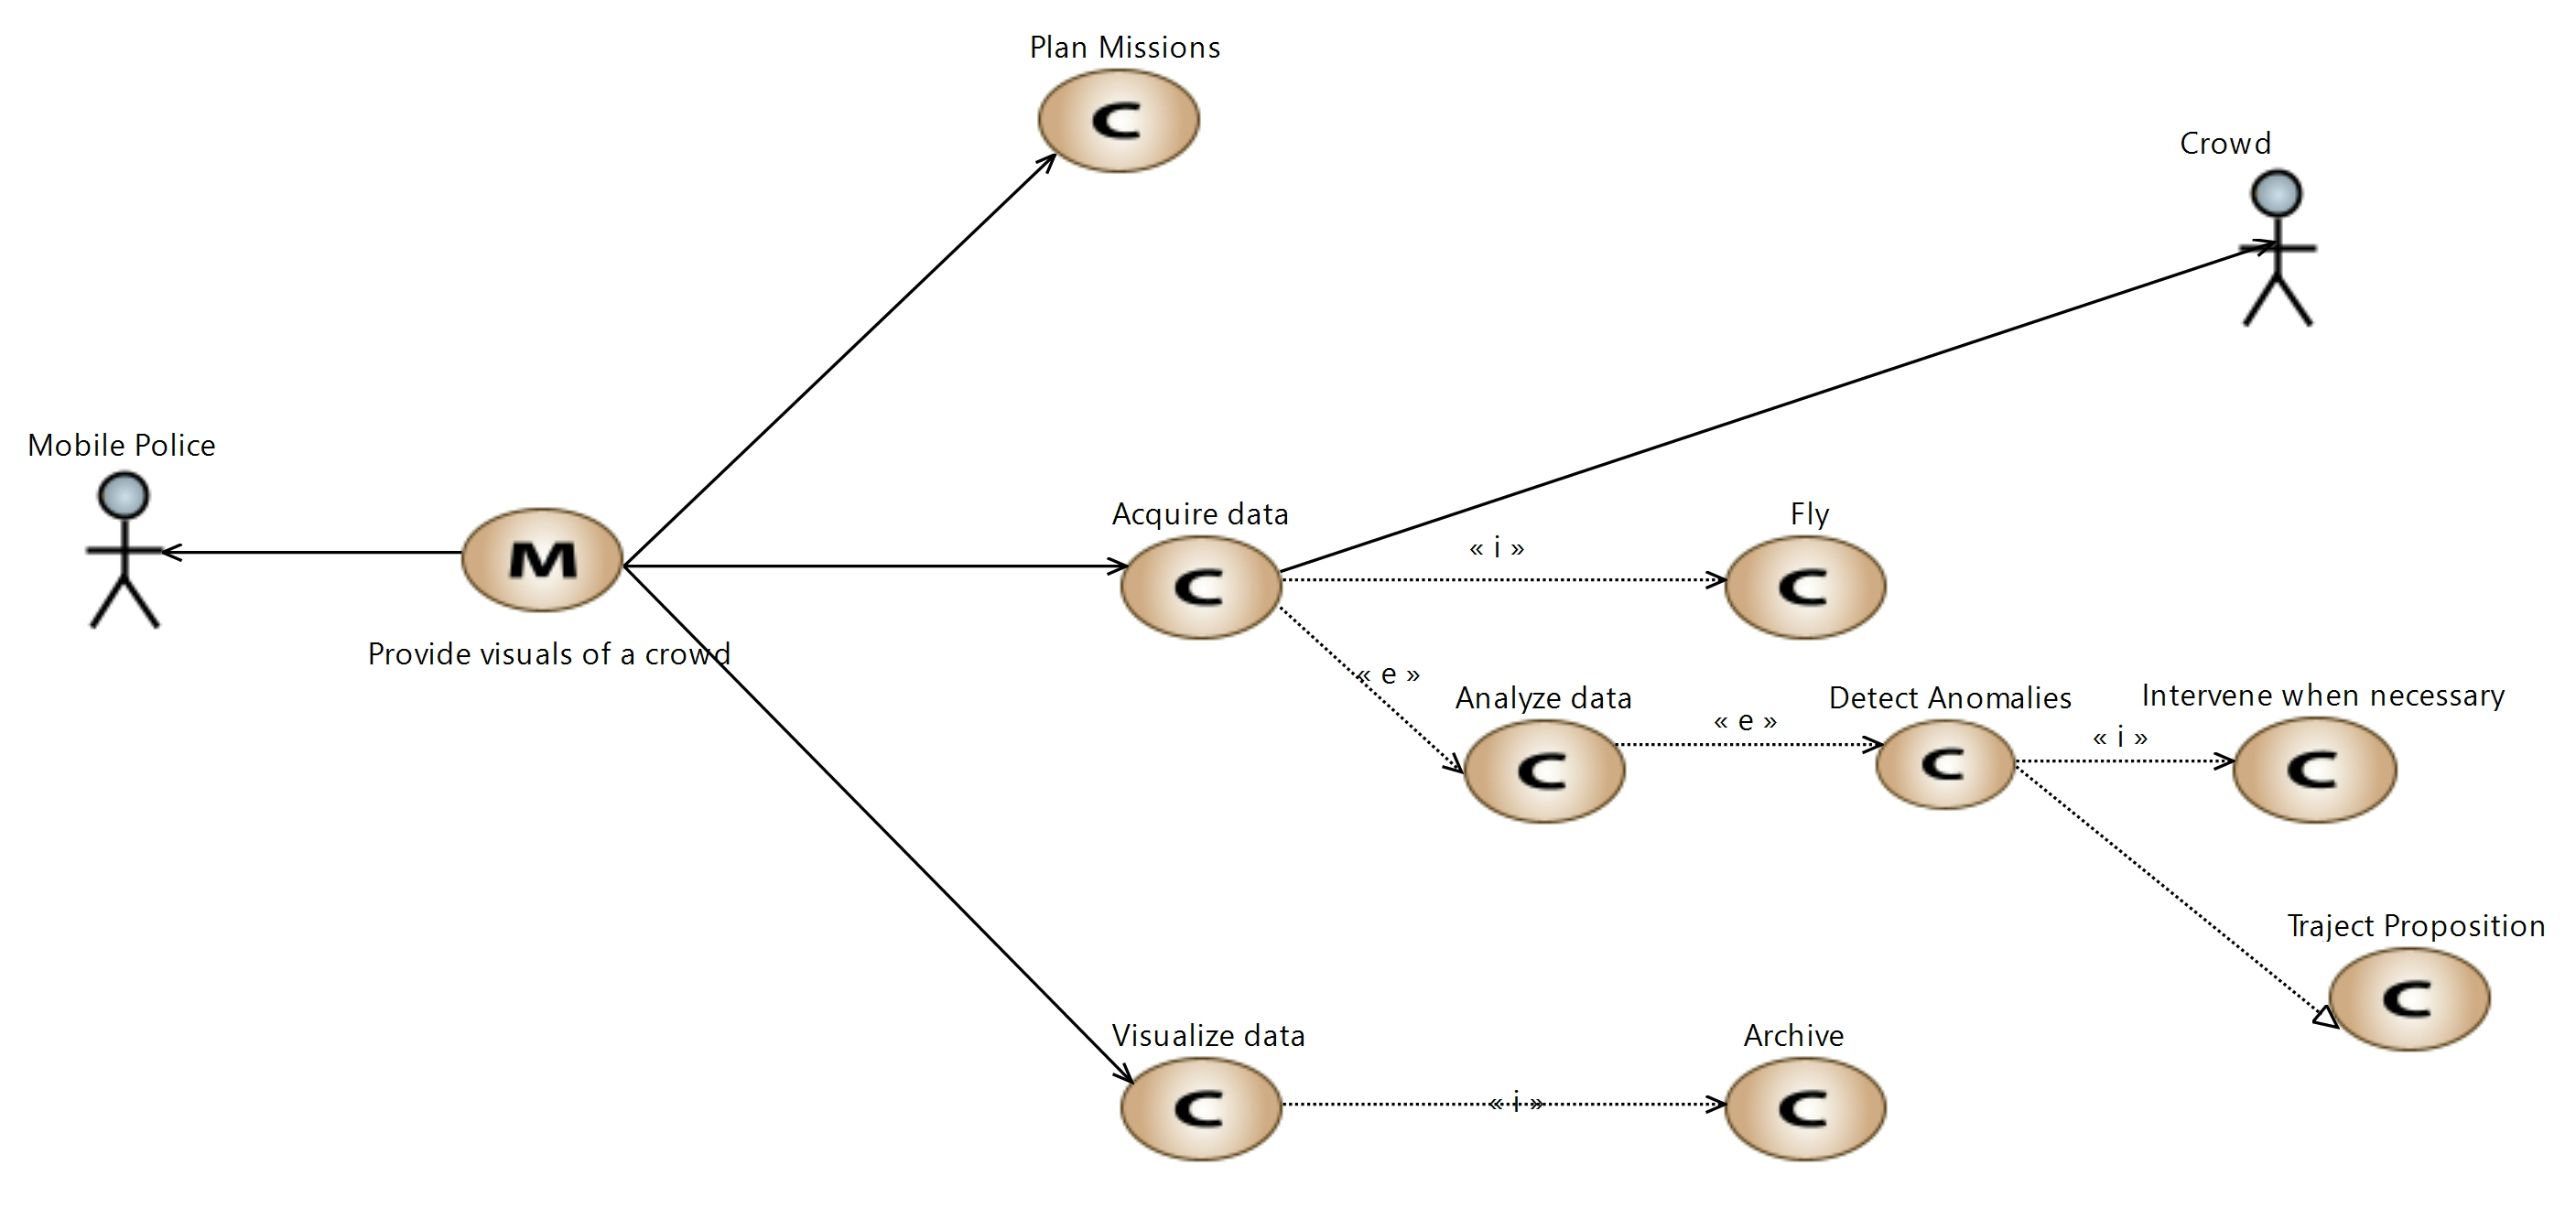
\includegraphics[width=\textwidth, height=6.75cm, keepaspectratio]{./images/EX2/CSC_5RO08_TA_EX2_MCB_High.jpg}
            % \caption{}
        \end{figure}
    \end{frame}
    \begin{frame}{Exercice 2, MCB - Hybride Performance}
        \begin{figure}[H]
            \centering
            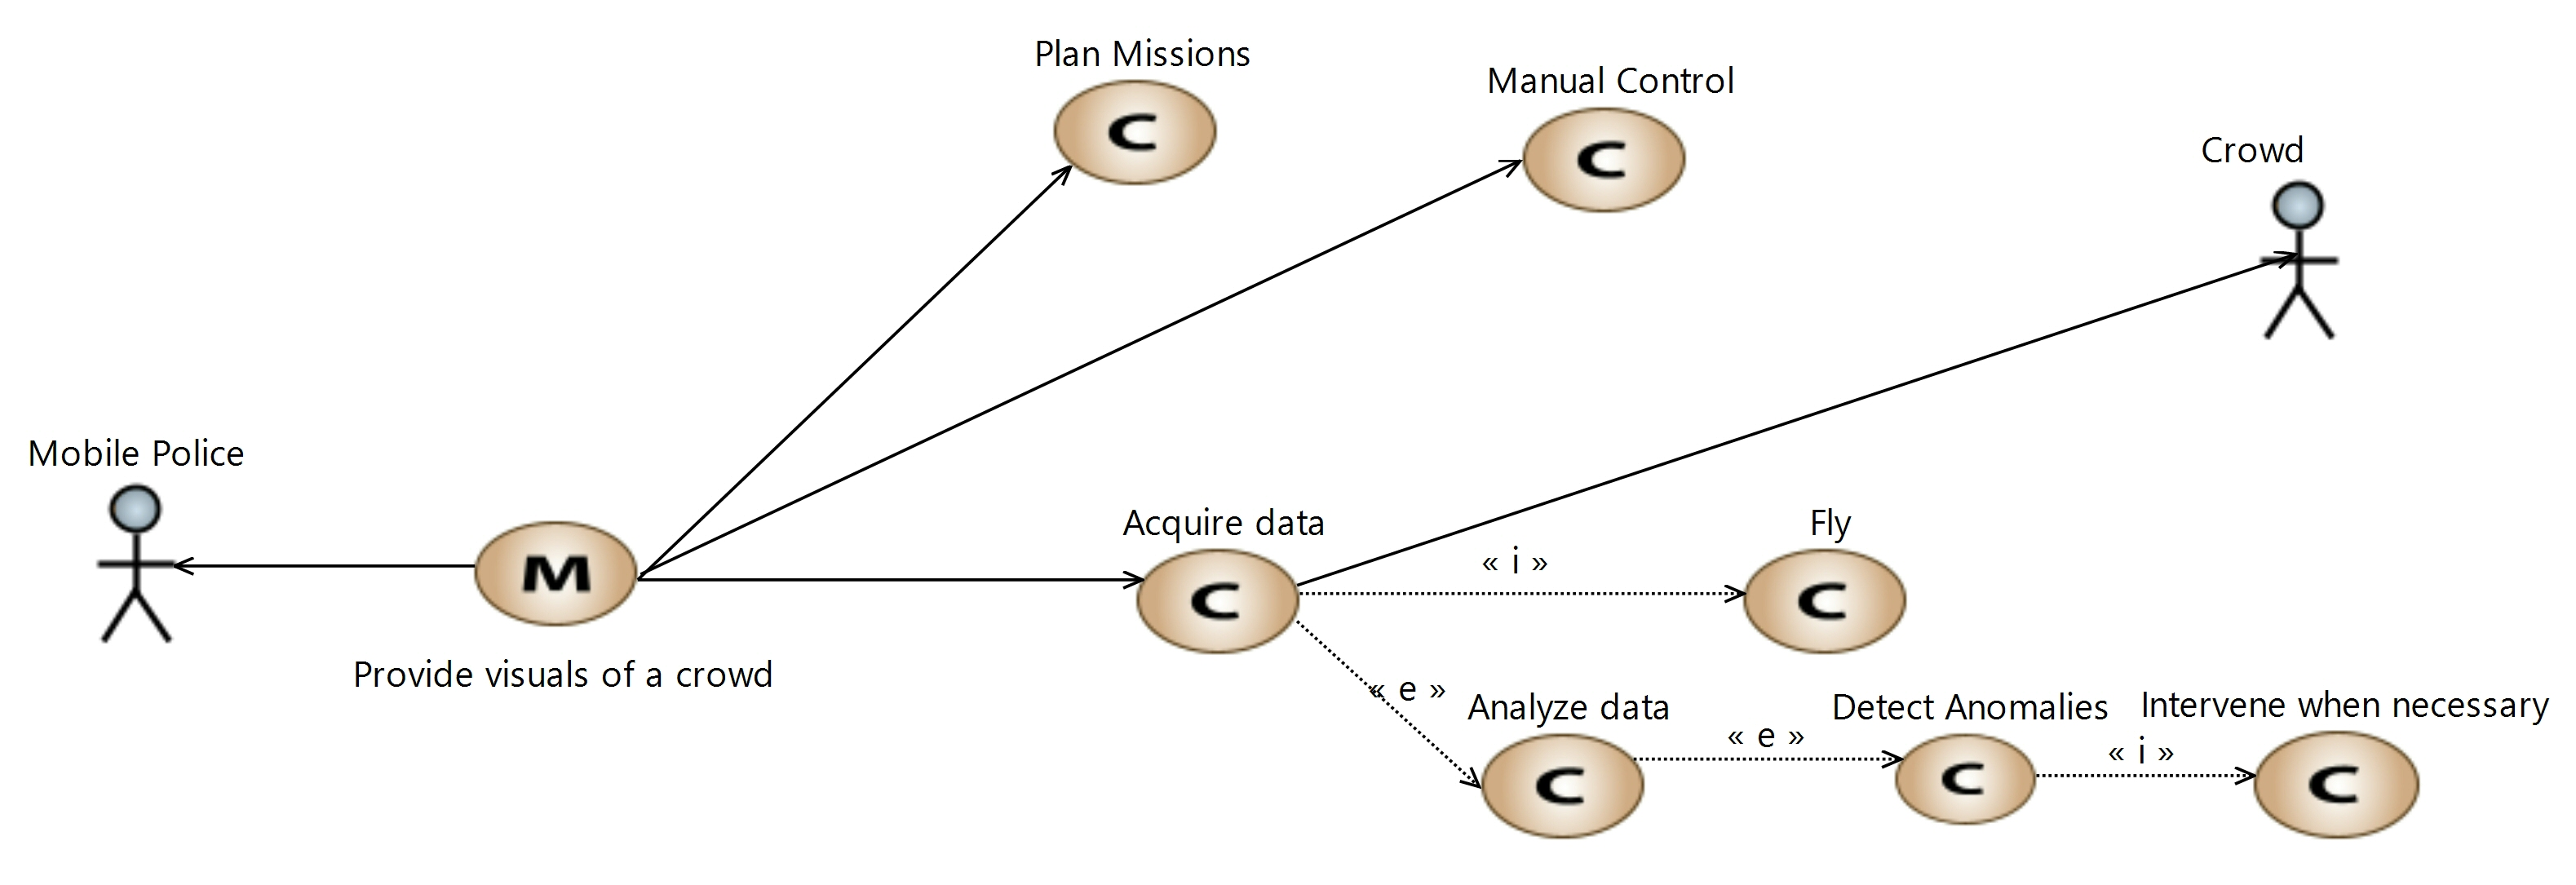
\includegraphics[width=\textwidth, height=6.75cm, keepaspectratio]{./images/EX2/CSC_5RO08_TA_EX2_MCB_Hybride.jpg}
            % \caption{}
        \end{figure}
    \end{frame}
    \begin{frame}{Exercice 2, MCB - Low Performance}
        \begin{figure}[H]
            \centering
            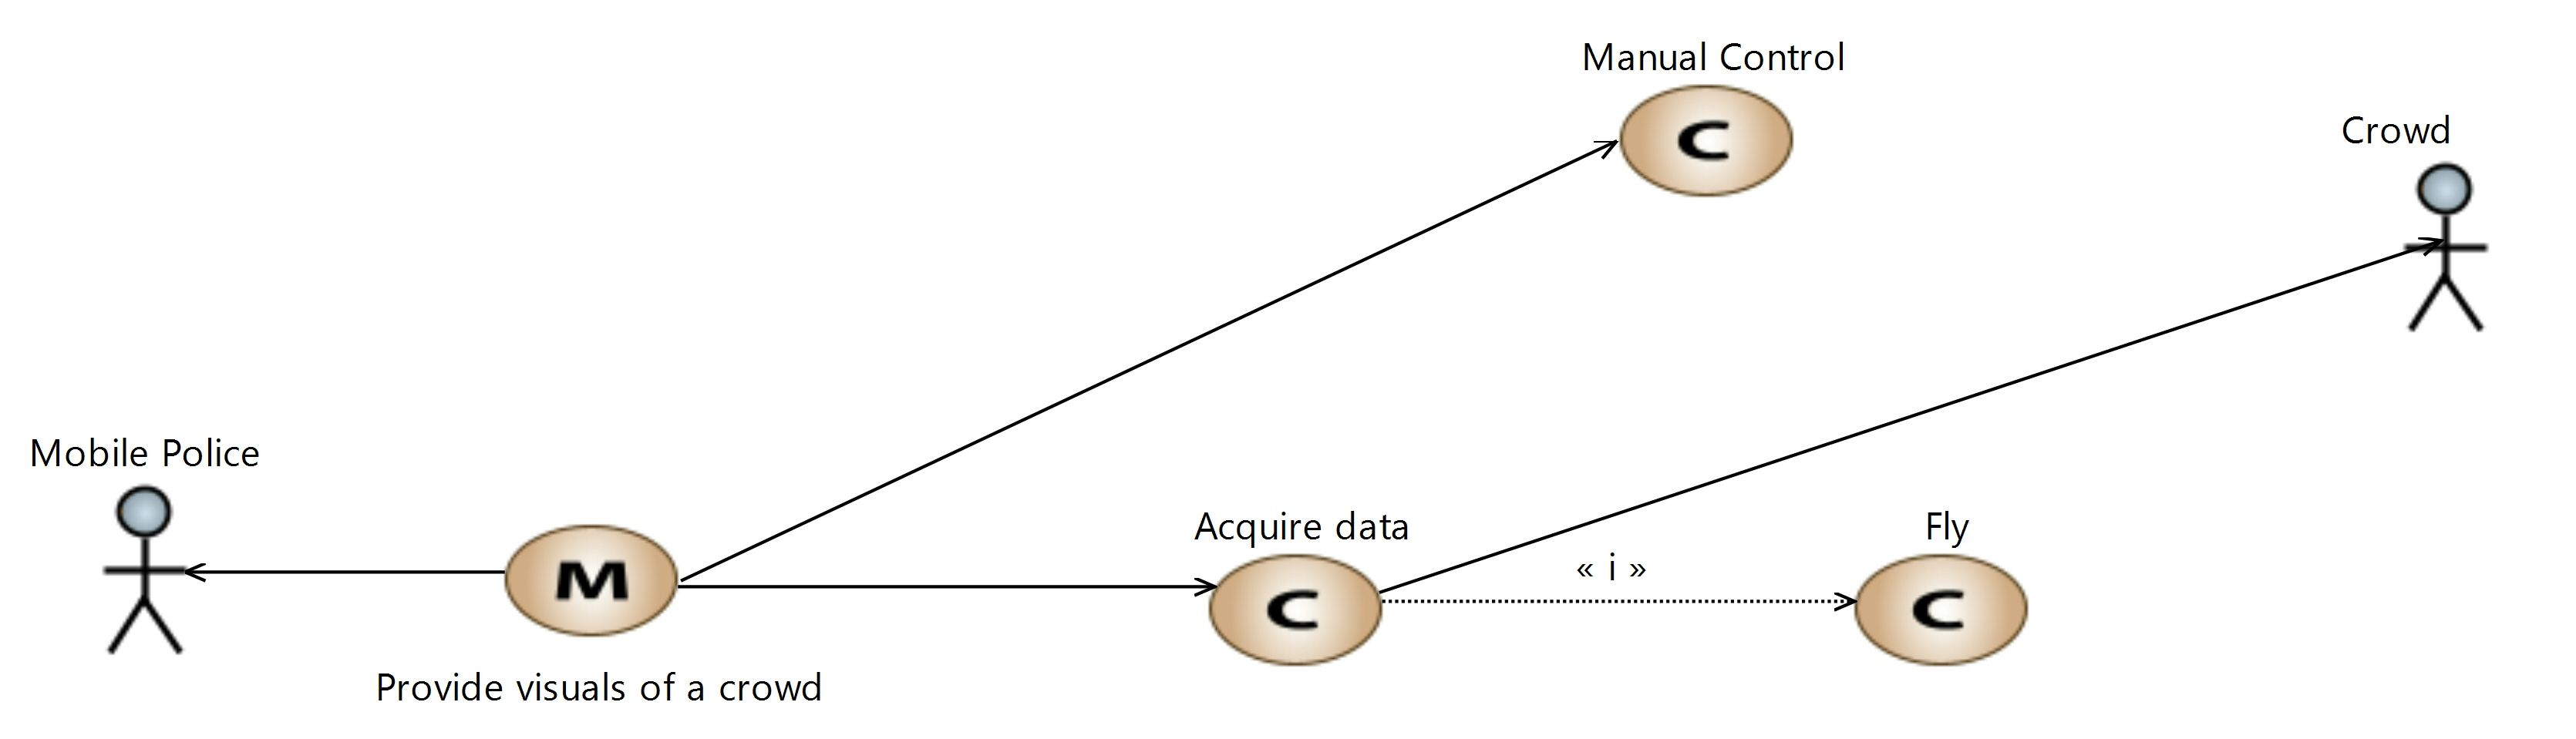
\includegraphics[width=\textwidth, height=6.75cm, keepaspectratio]{./images/EX2/CSC_5RO08_TA_EX2_MCB_Low.jpg}
            % \caption{}
        \end{figure}
    \end{frame}

    \subsection{System Architecture Blank}
    \begin{frame}{Exercice 2, System Architecture Blank}
        \begin{figure}[H]
            \centering
            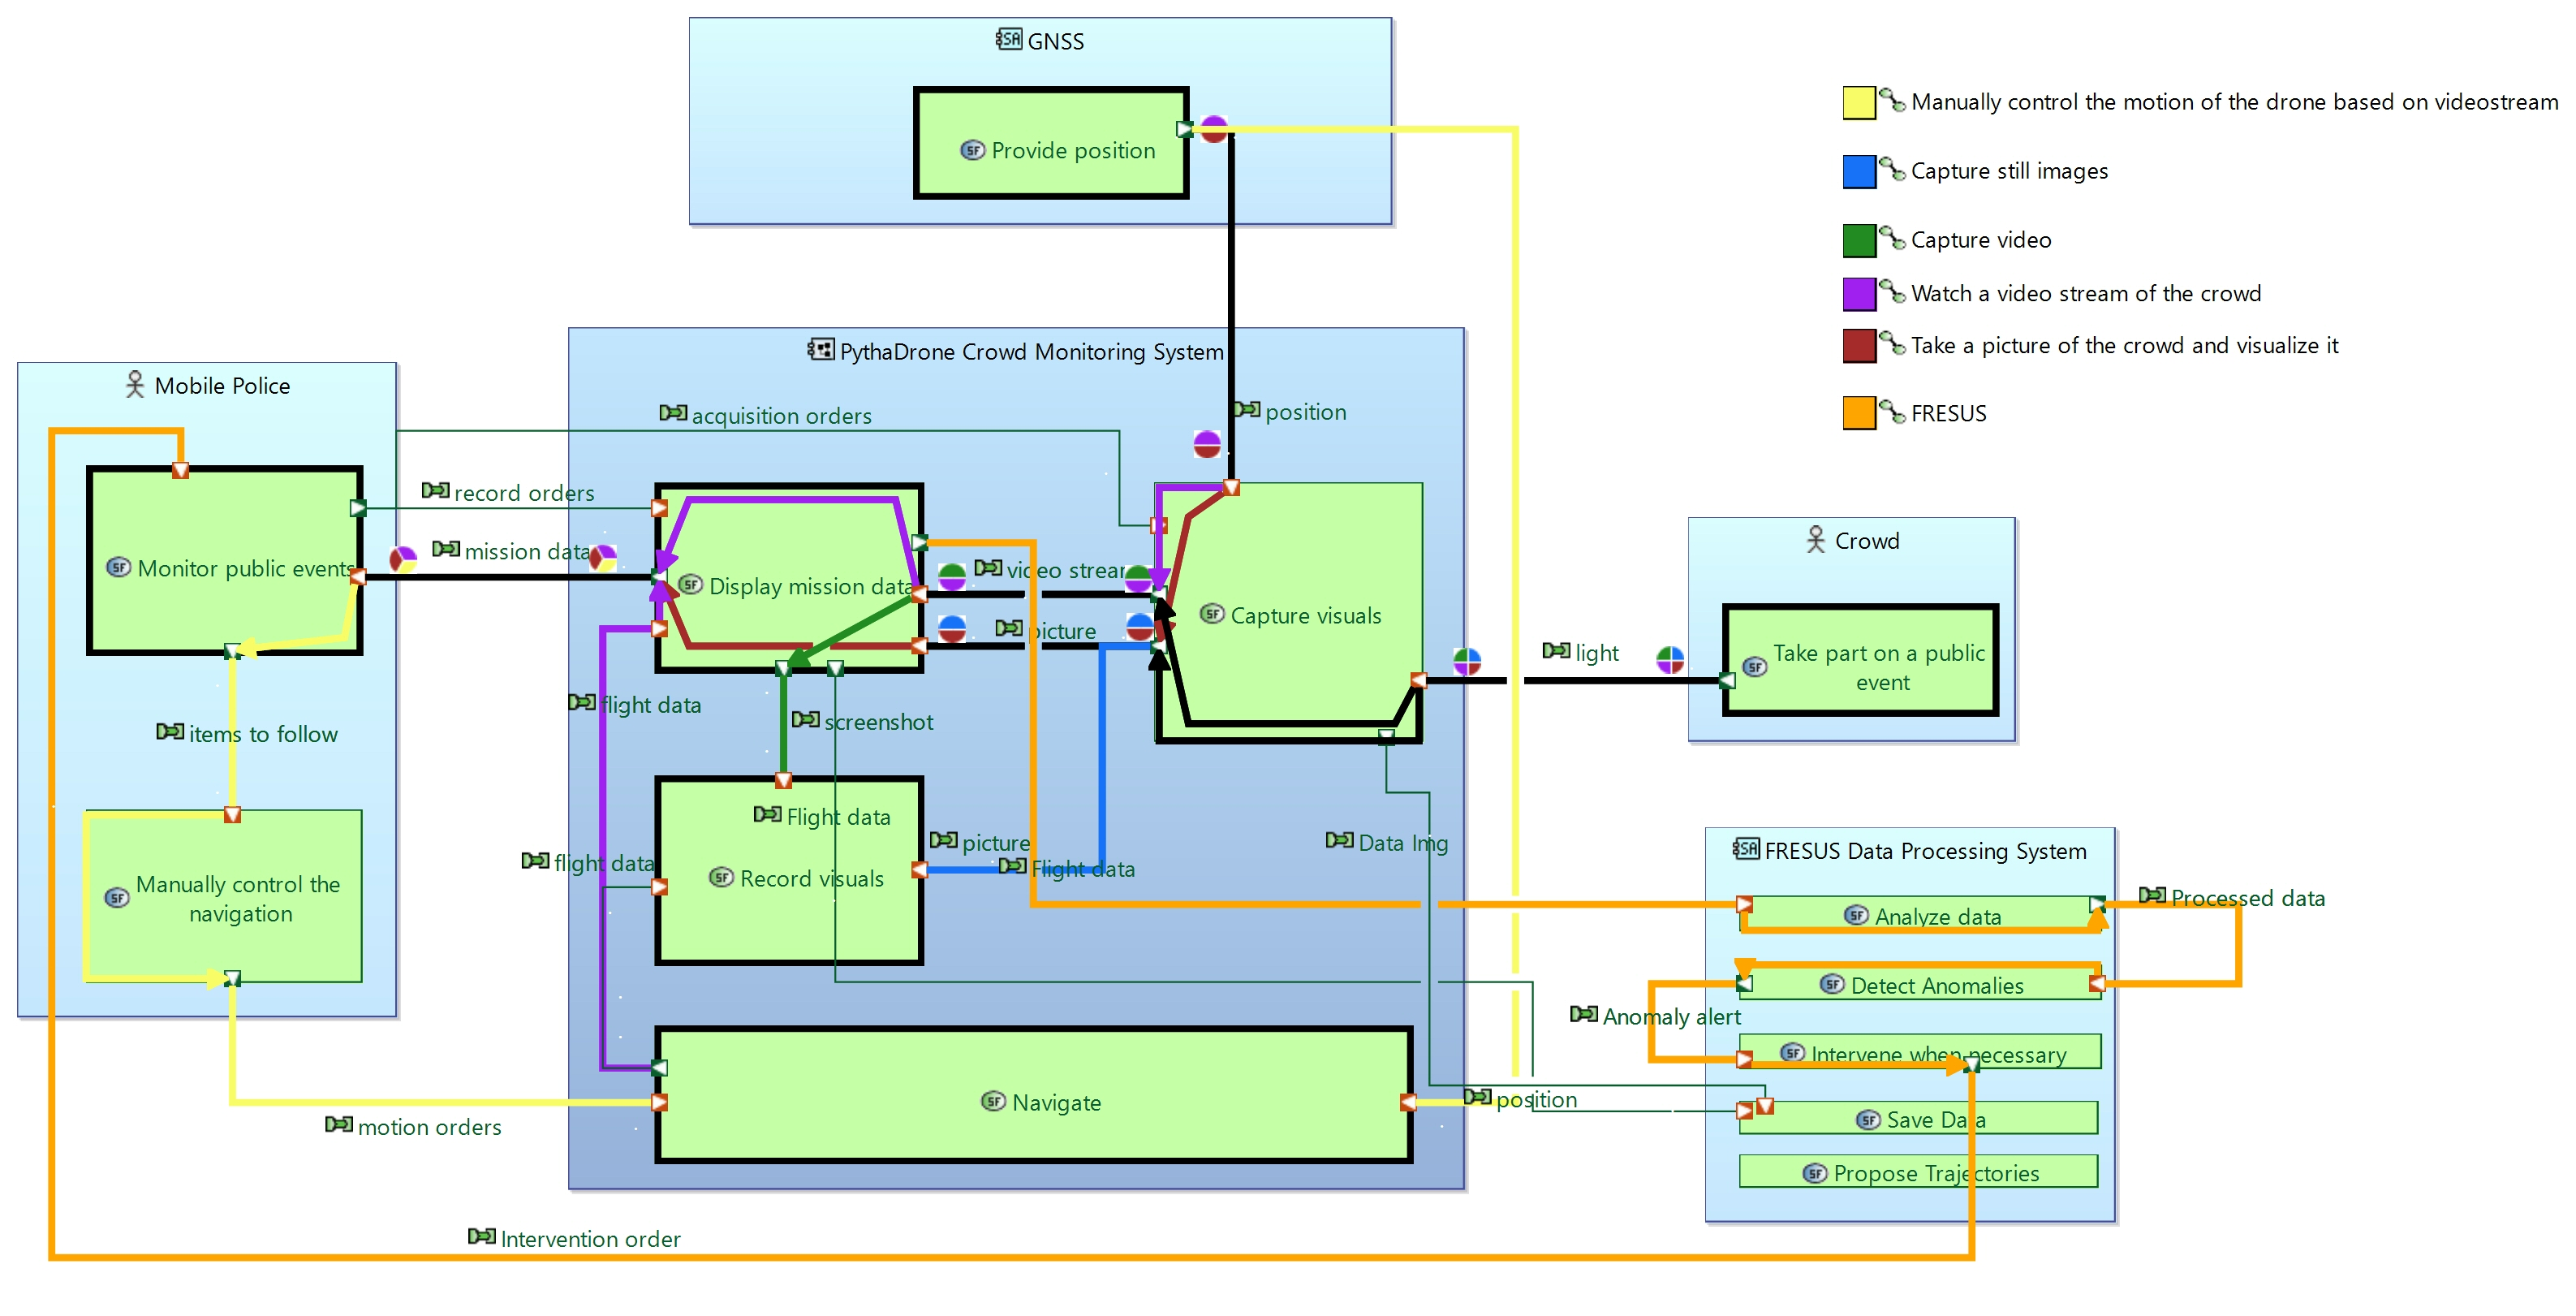
\includegraphics[width=\textwidth, height=6.75cm, keepaspectratio]{./images/EX2/CSC_5RO08_TA_EX2_SAB.jpg}
            % \caption{}
        \end{figure}
    \end{frame}
    \begin{frame}{Exercice 2, System Architecture Blank - High Performance}
        \begin{figure}[H]
            \centering
            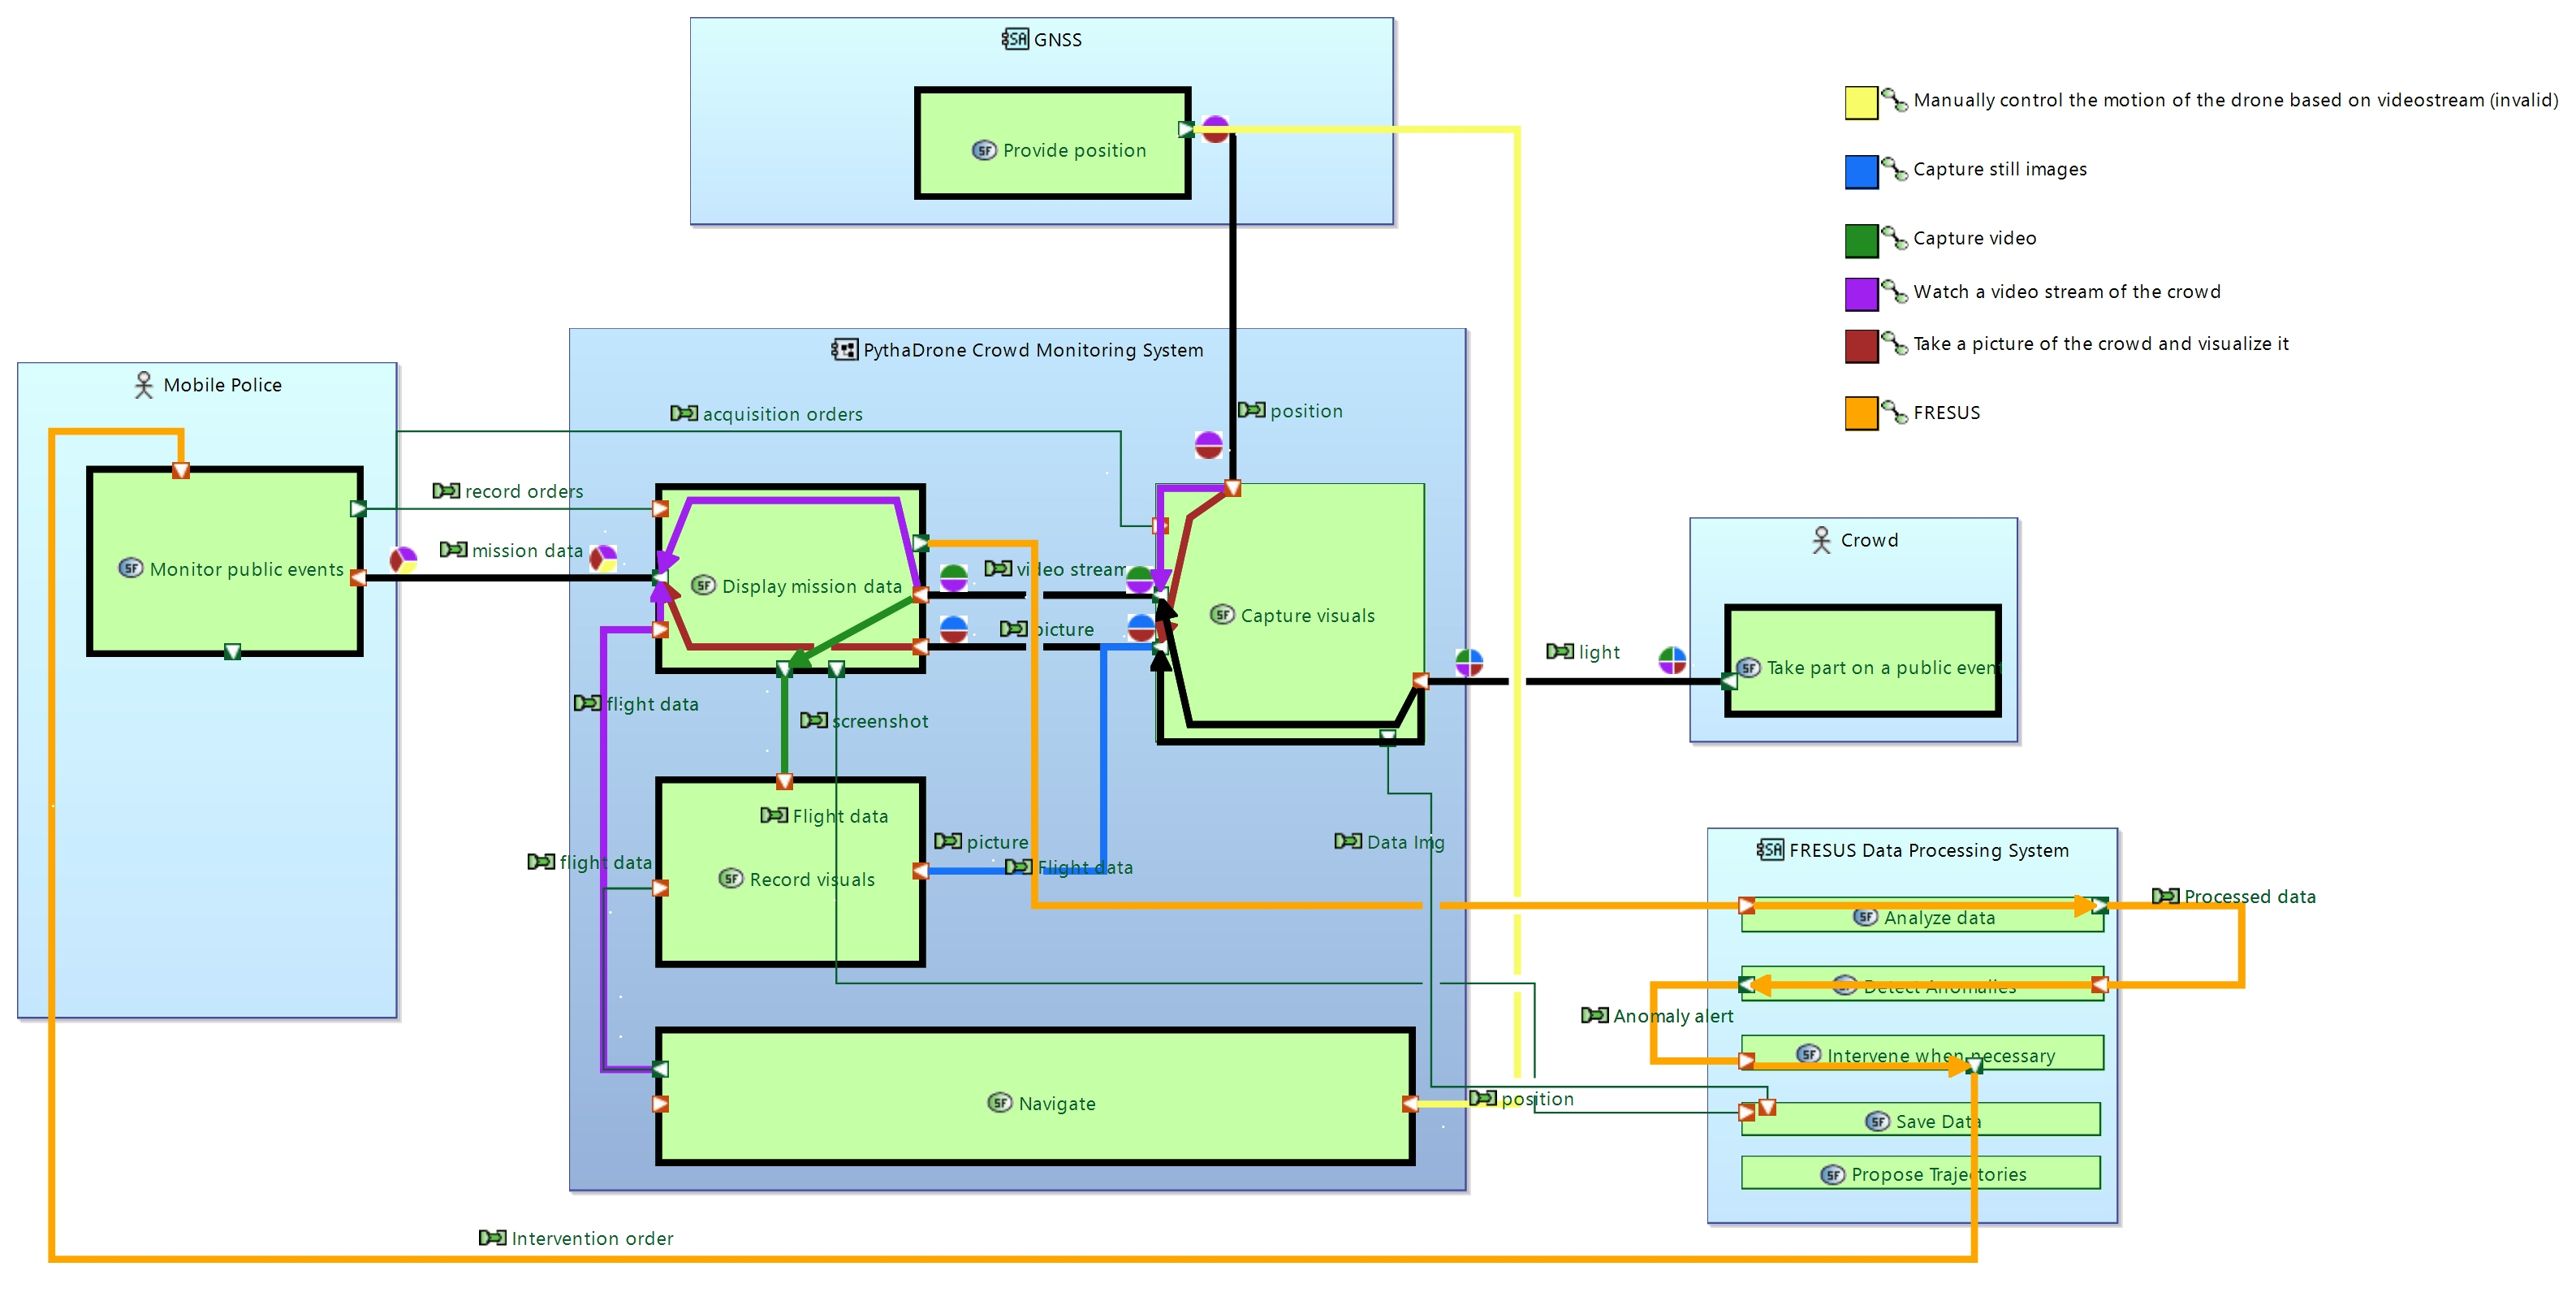
\includegraphics[width=\textwidth, height=6.75cm, keepaspectratio]{./images/EX2/CSC_5RO08_TA_EX2_SAB_High.jpg}
            % \caption{}
        \end{figure}
    \end{frame}
    \begin{frame}{Exercice 2, System Architecture Blank - Hybride Performance}
        \begin{figure}[H]
            \centering
            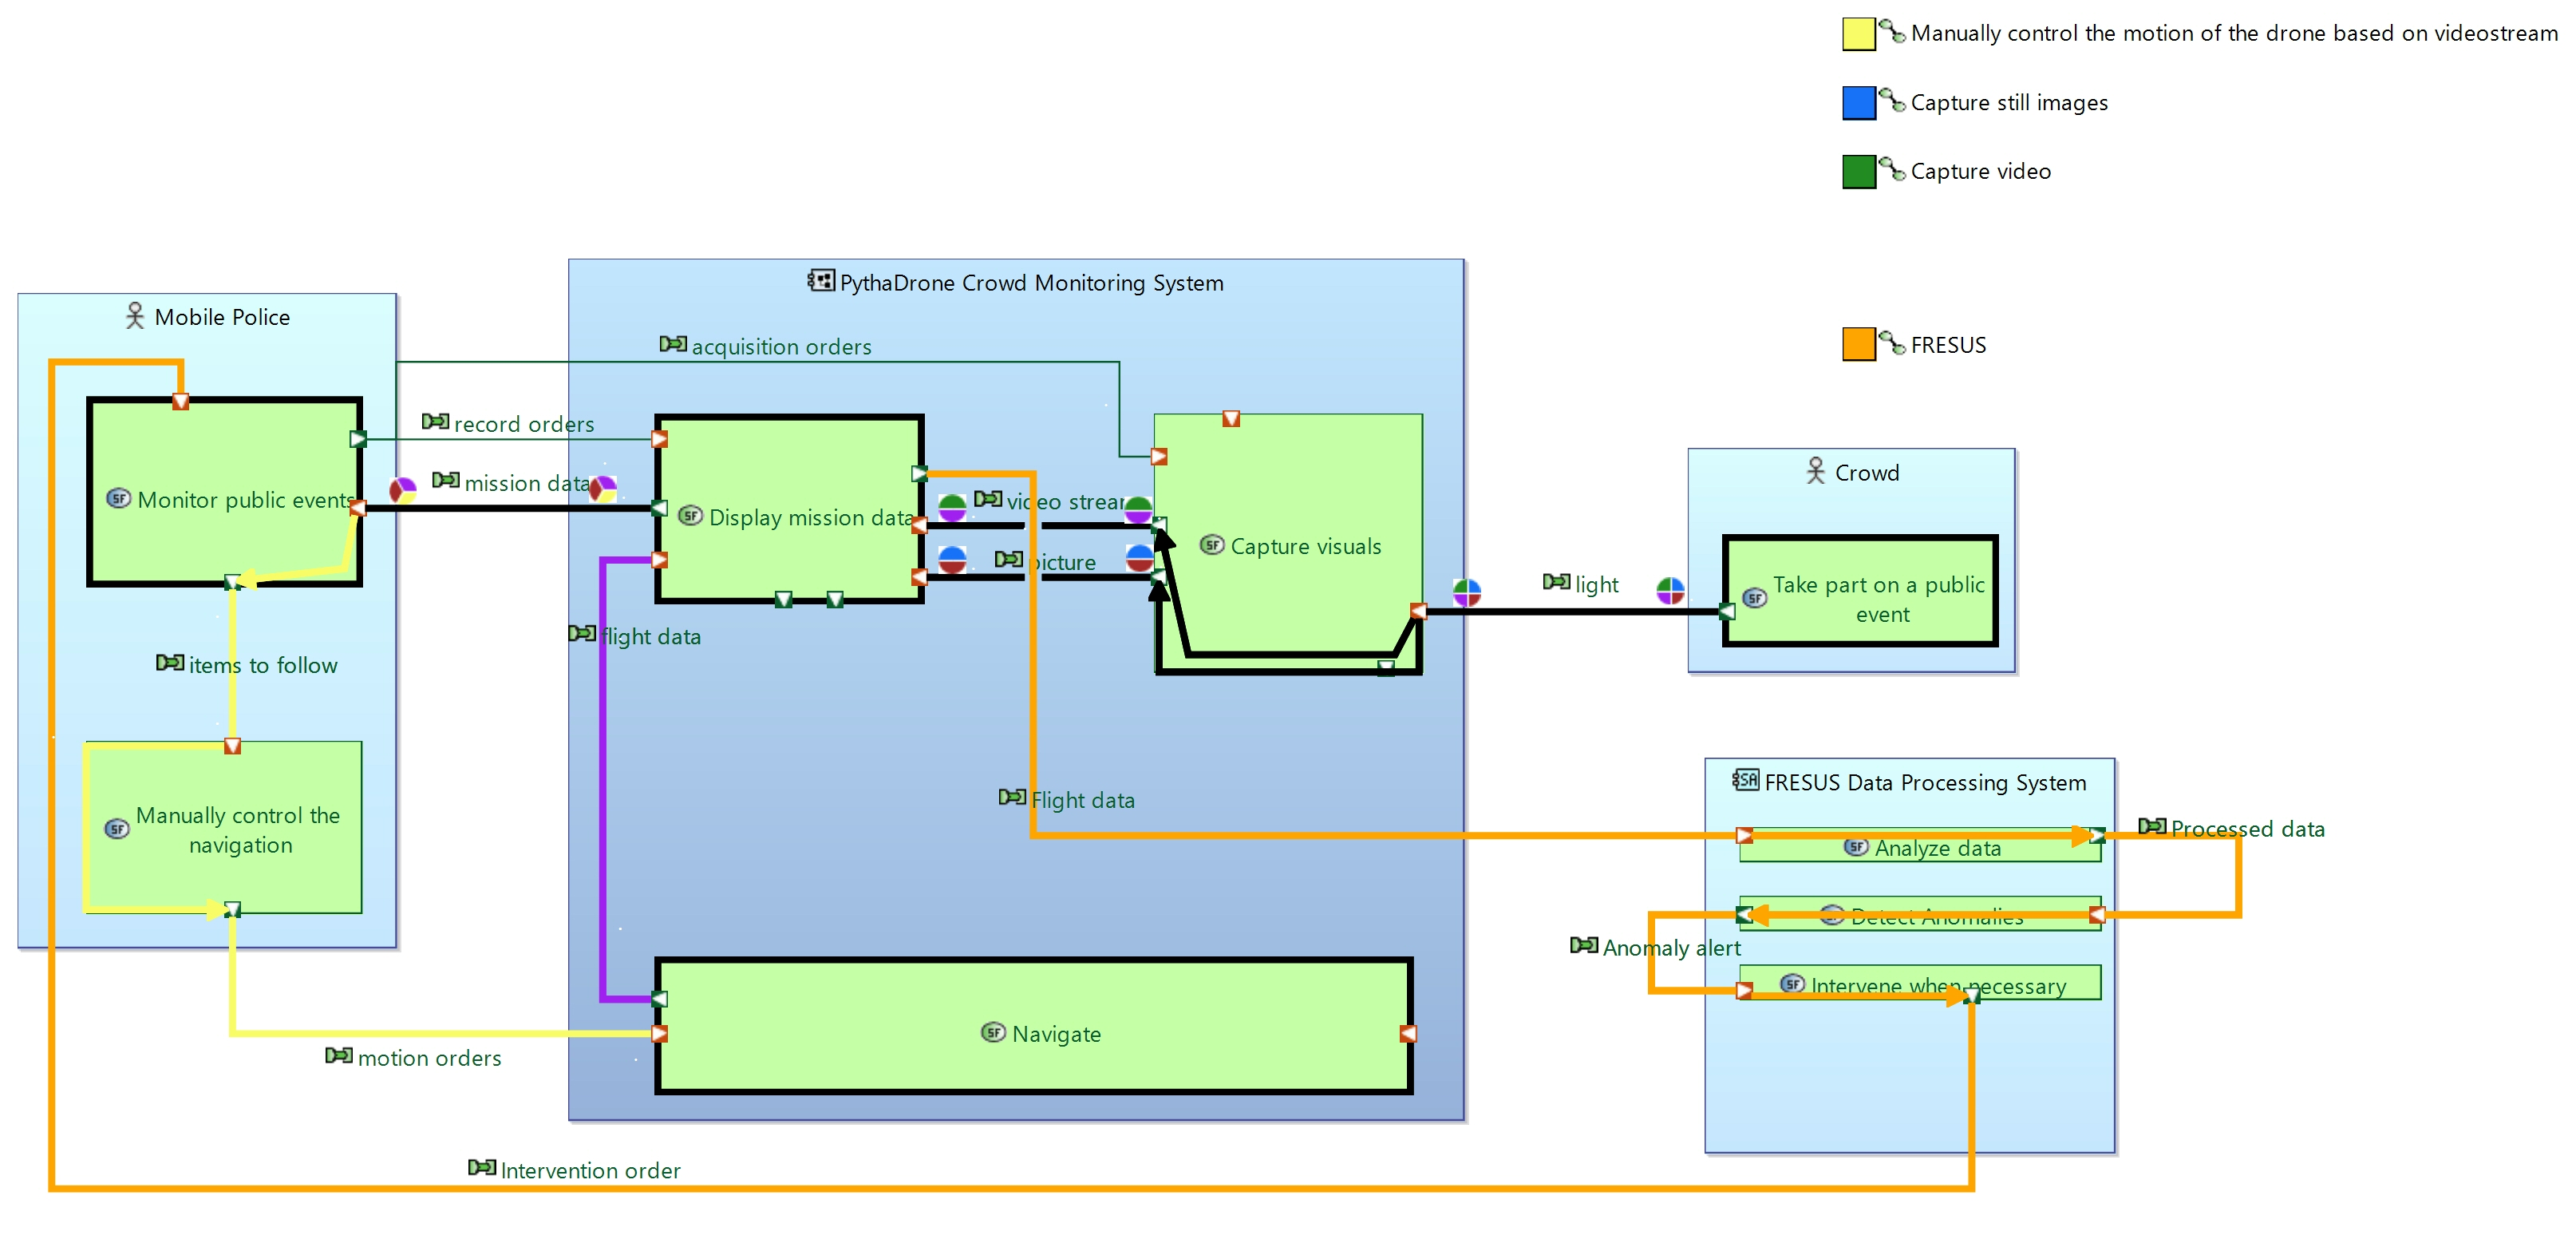
\includegraphics[width=\textwidth, height=6.75cm, keepaspectratio]{./images/EX2/CSC_5RO08_TA_EX2_SAB_Hybride.jpg}
            % \caption{}
        \end{figure}
    \end{frame}
    \begin{frame}{Exercice 2, System Architecture Blank - Low Performance}
        \begin{figure}[H]
            \centering
            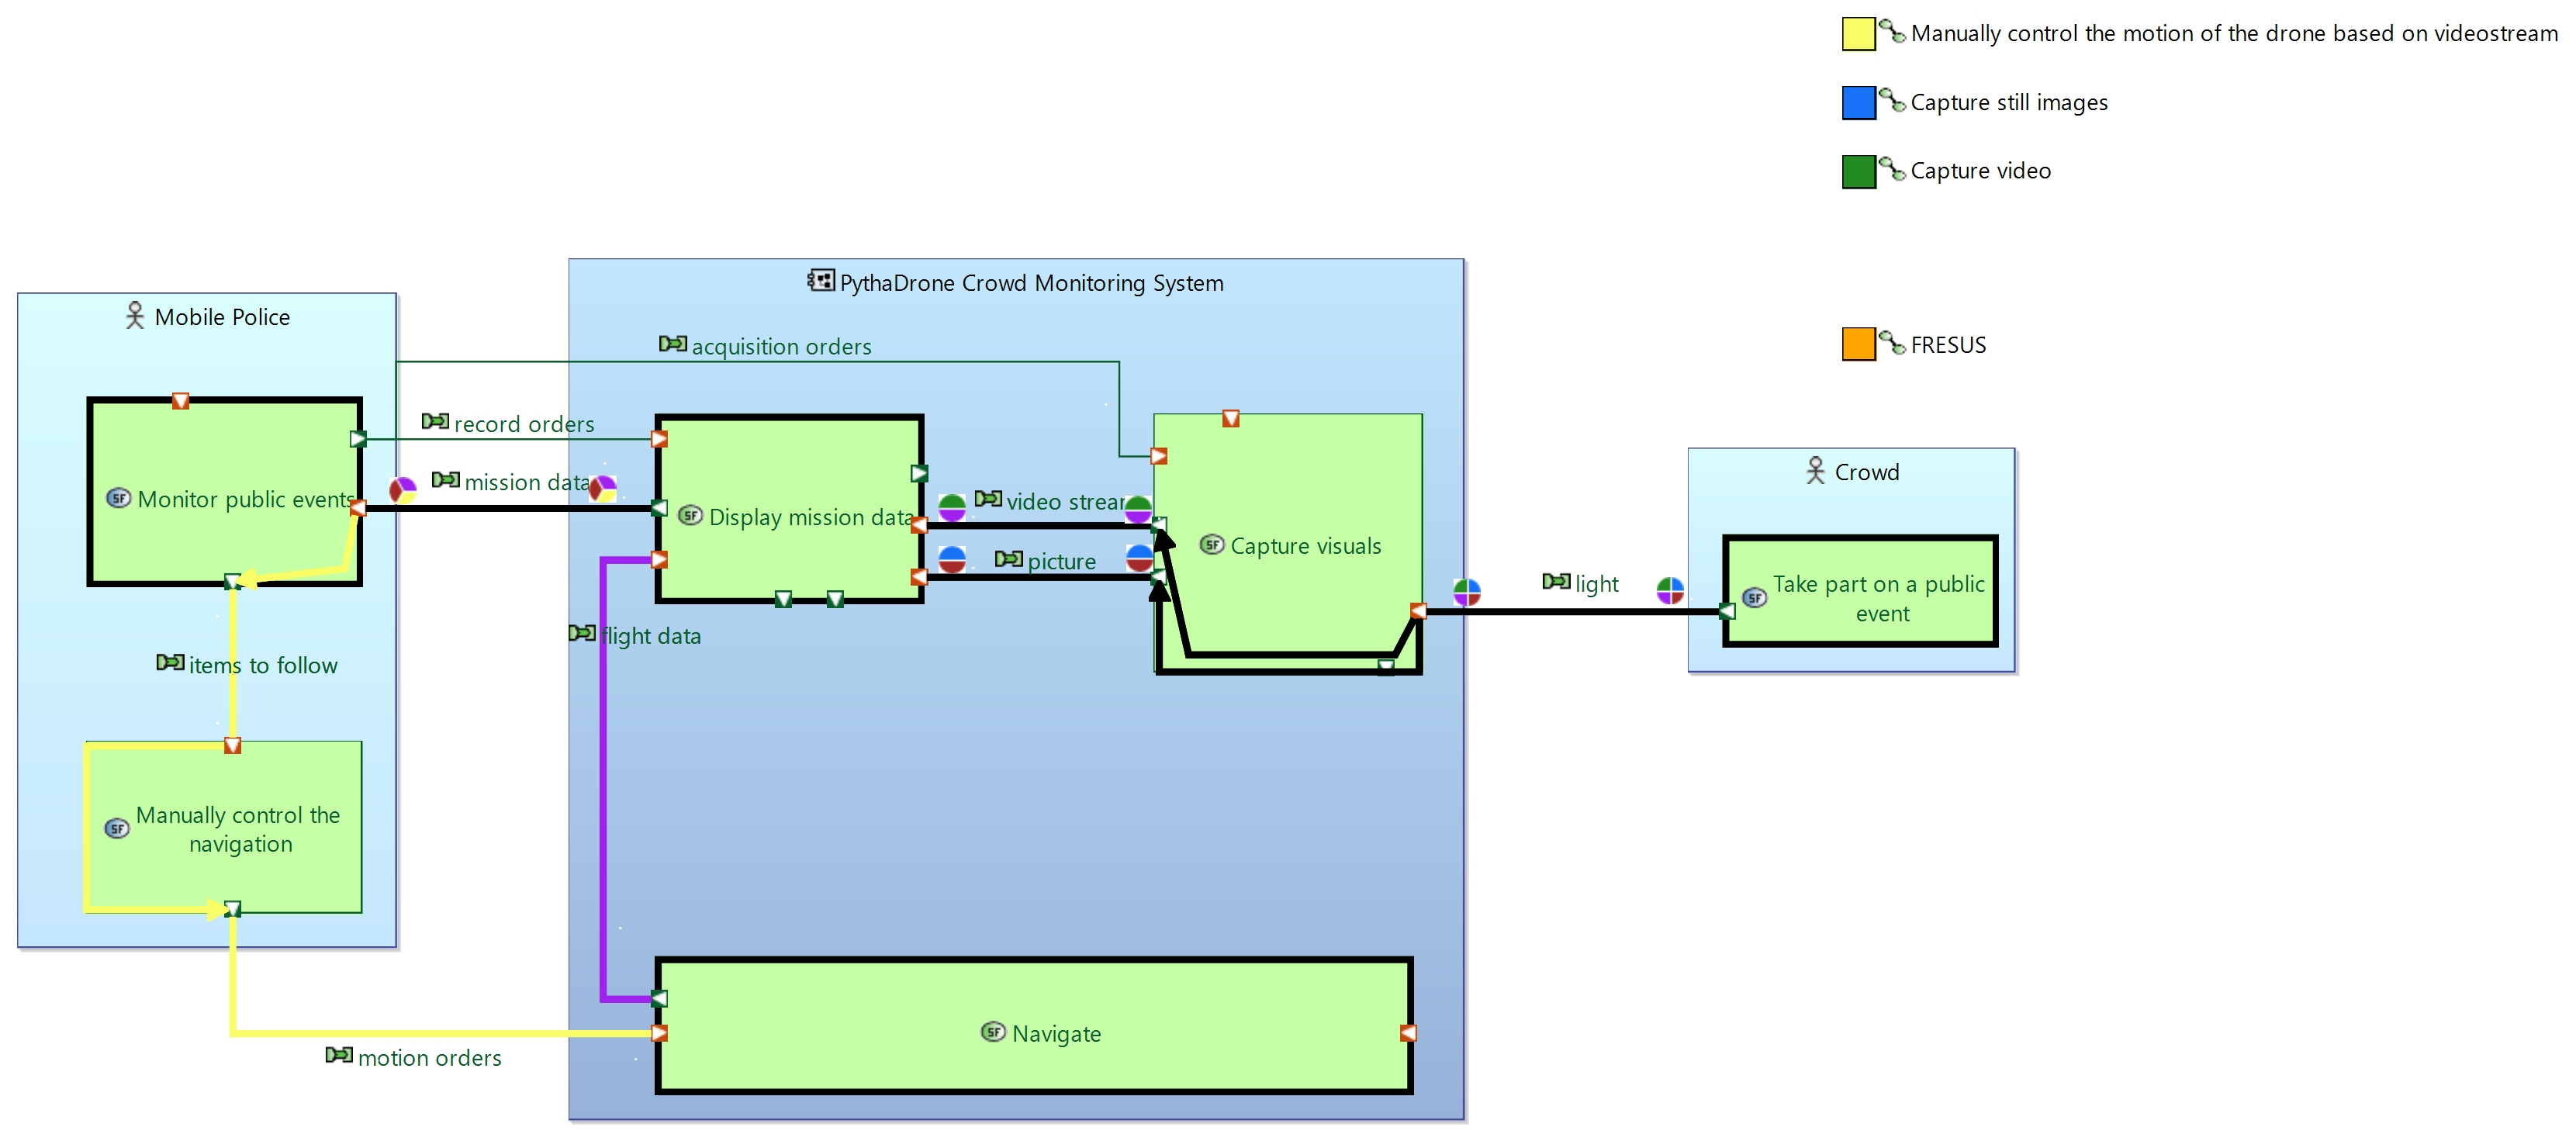
\includegraphics[width=\textwidth, height=6.75cm, keepaspectratio]{./images/EX2/CSC_5RO08_TA_EX2_SAB_Low.jpg}
            % \caption{}
        \end{figure}
    \end{frame}

    \subsection{Physical Architecture Blank}
    \begin{frame}{Exercice 2, Physical Architecture Blank}
        \begin{figure}[H]
            \centering
            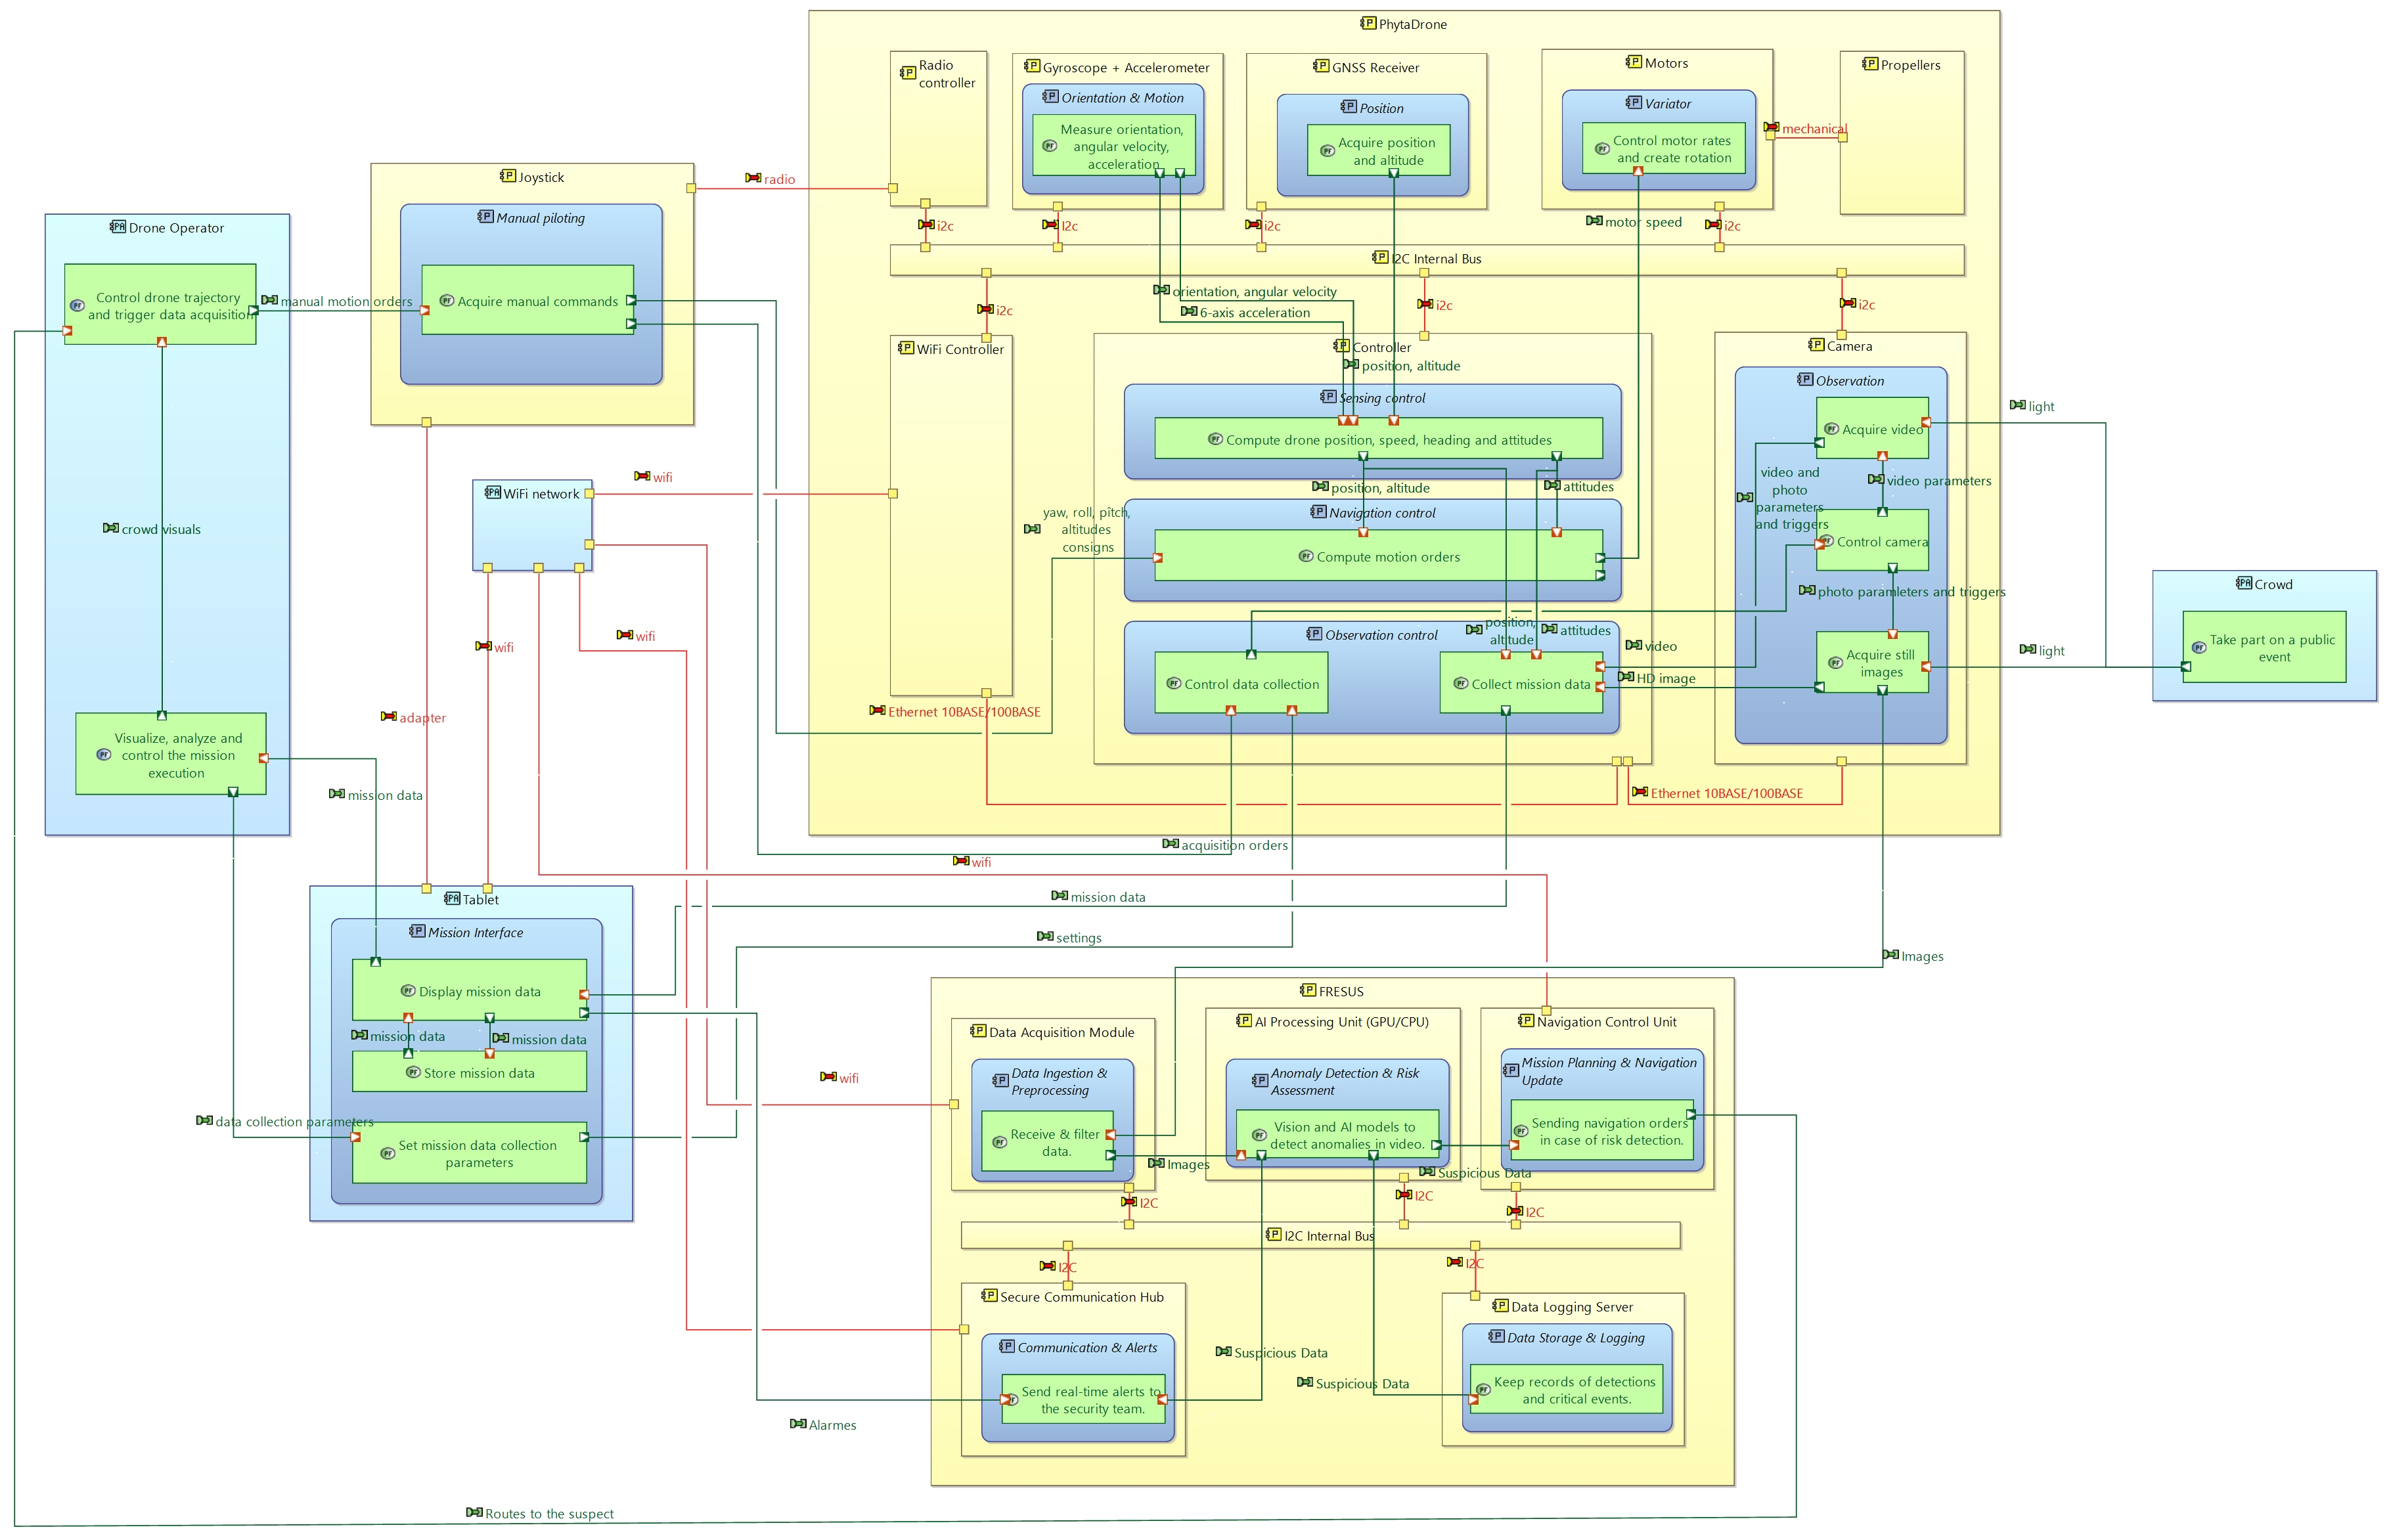
\includegraphics[width=\textwidth, height=6.75cm, keepaspectratio]{./images/EX2/CSC_5RO08_TA_EX2_PAB_Original.jpg}
            % \caption{}
        \end{figure}
    \end{frame}
    \begin{frame}{Exercice 2, Physical Architecture Blank - High Performance}
        \begin{figure}[H]
            \centering
            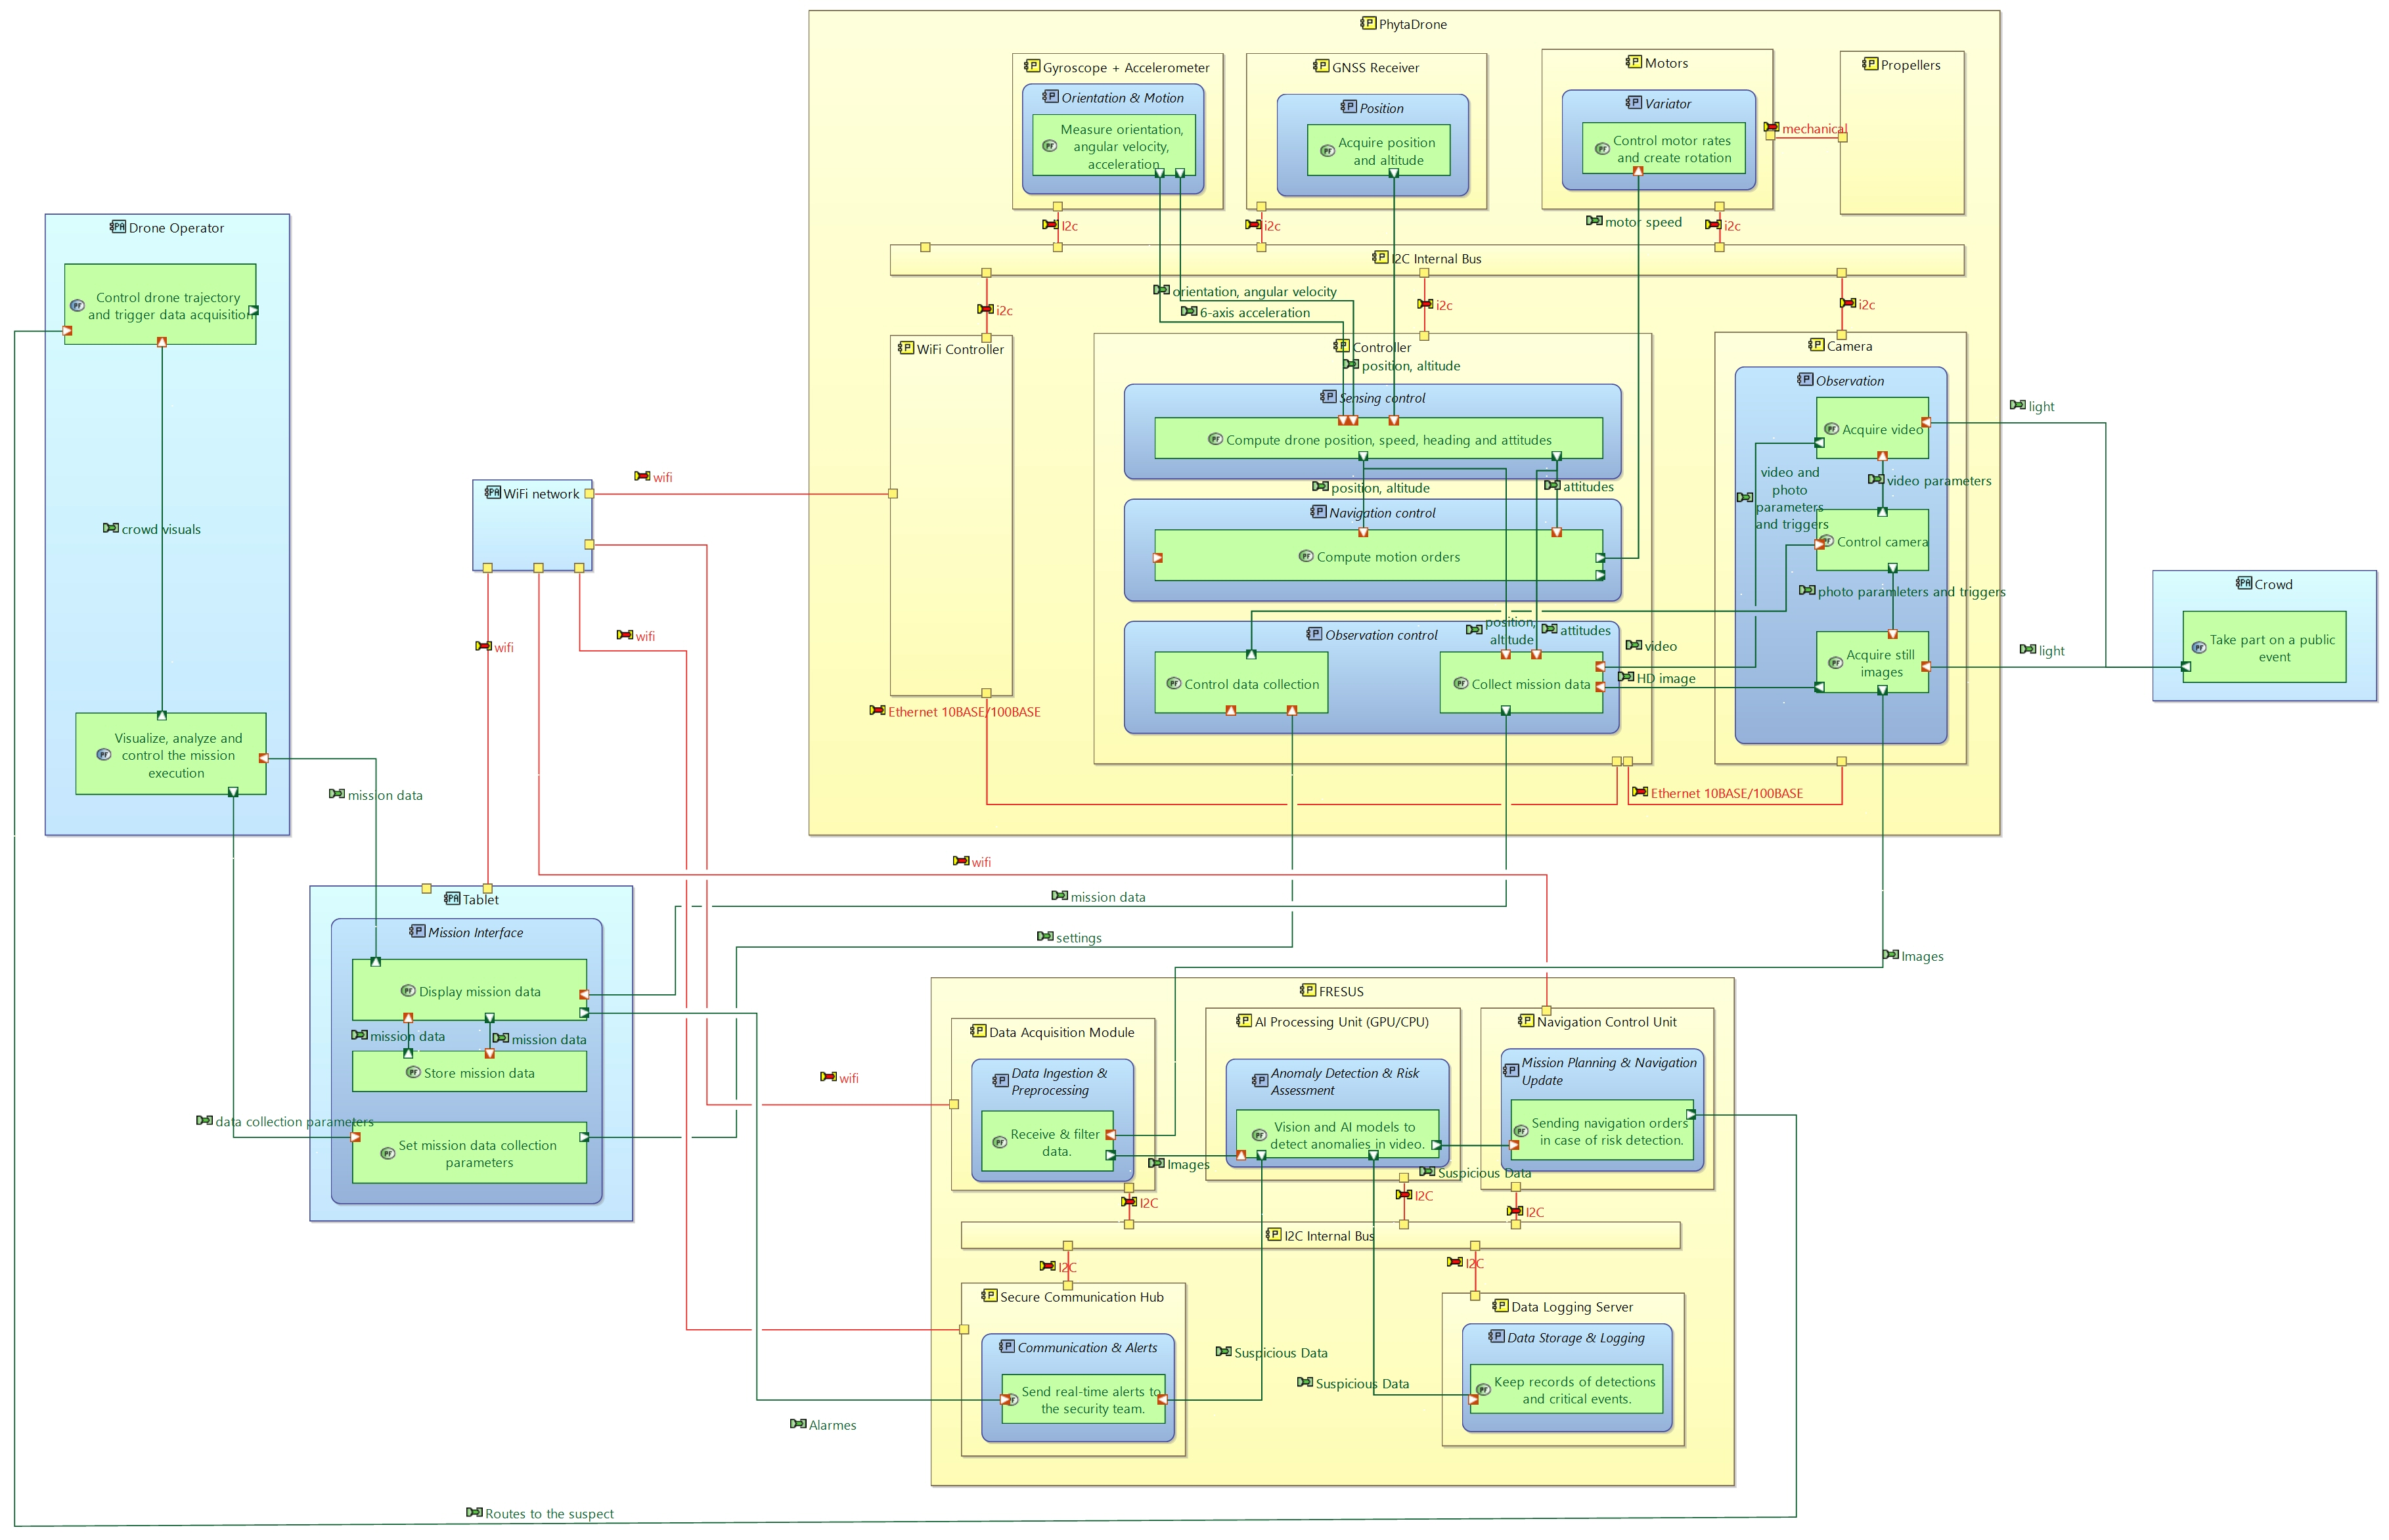
\includegraphics[width=\textwidth, height=6.75cm, keepaspectratio]{./images/EX2/CSC_5RO08_TA_EX2_PAB_High.jpg}
            % \caption{}
        \end{figure}
    \end{frame}
    \begin{frame}{Exercice 2, Physical Architecture Blank - Hybride Performance}
        \begin{figure}[H]
            \centering
            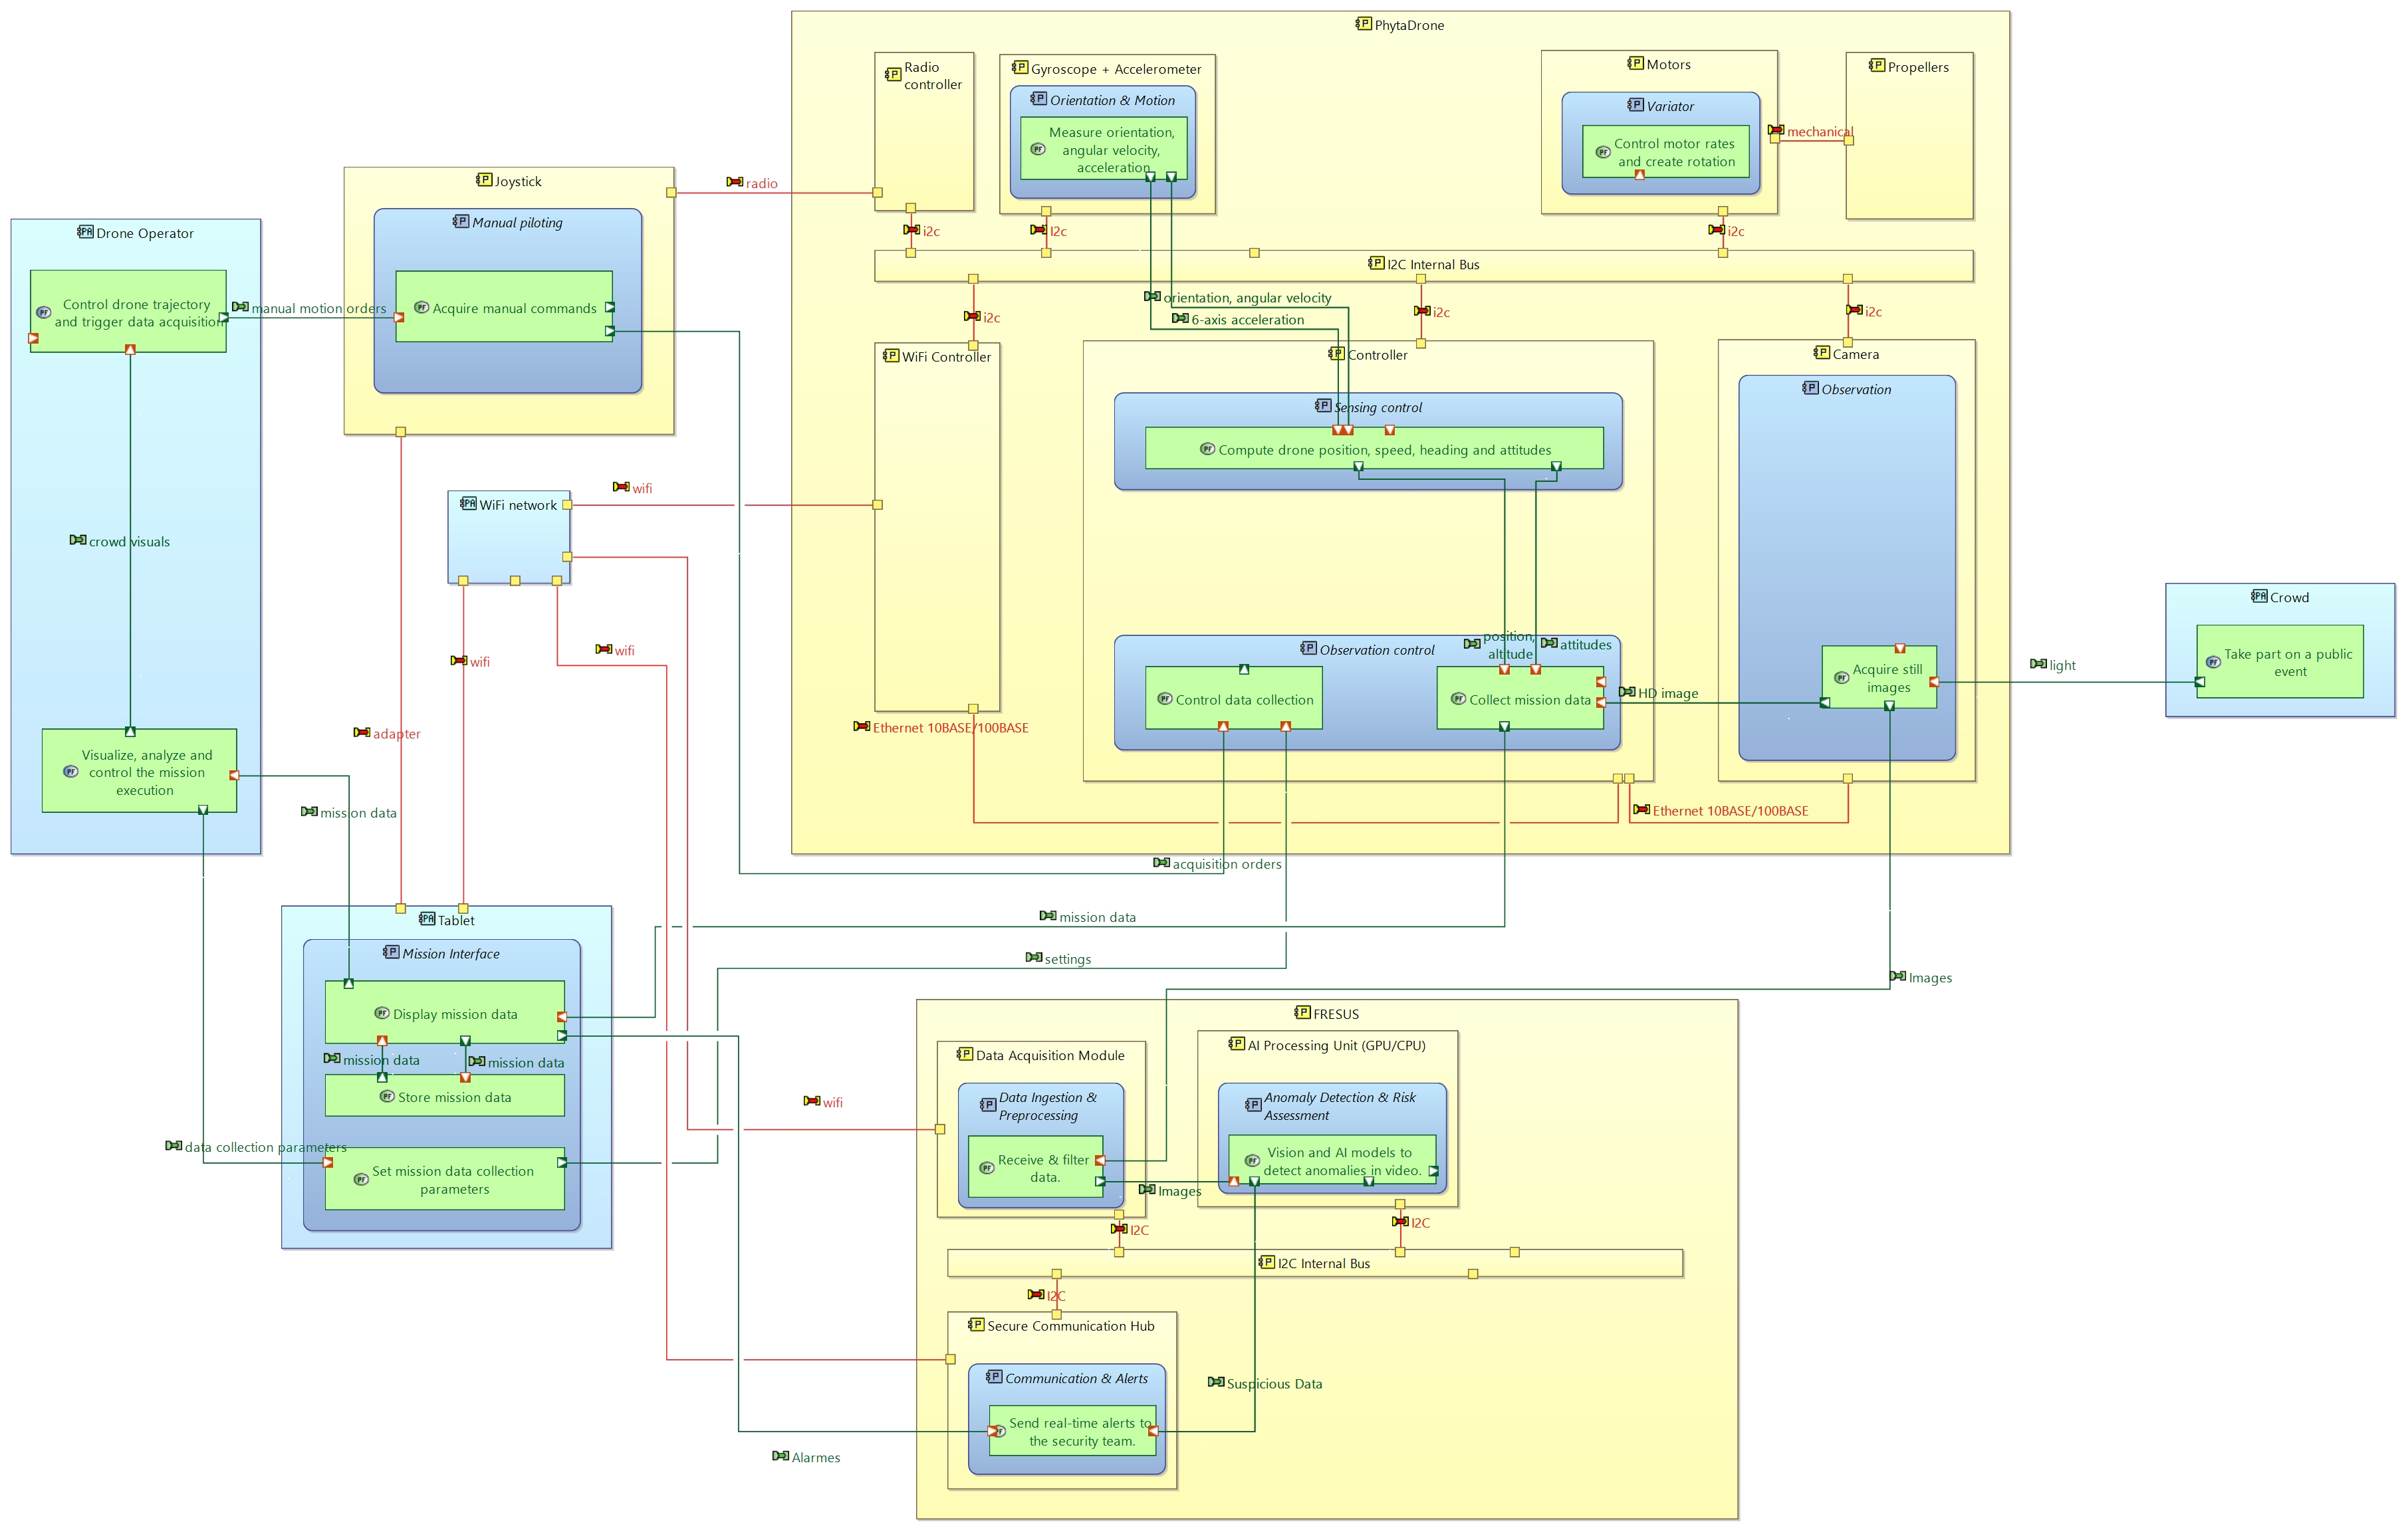
\includegraphics[width=\textwidth, height=6.75cm, keepaspectratio]{./images/EX2/CSC_5RO08_TA_EX2_PAB_Hybride.jpg}
            % \caption{}
        \end{figure}
    \end{frame}
    \begin{frame}{Exercice 2, Physical Architecture Blank - Low Performance}
        \begin{figure}[H]
            \centering
            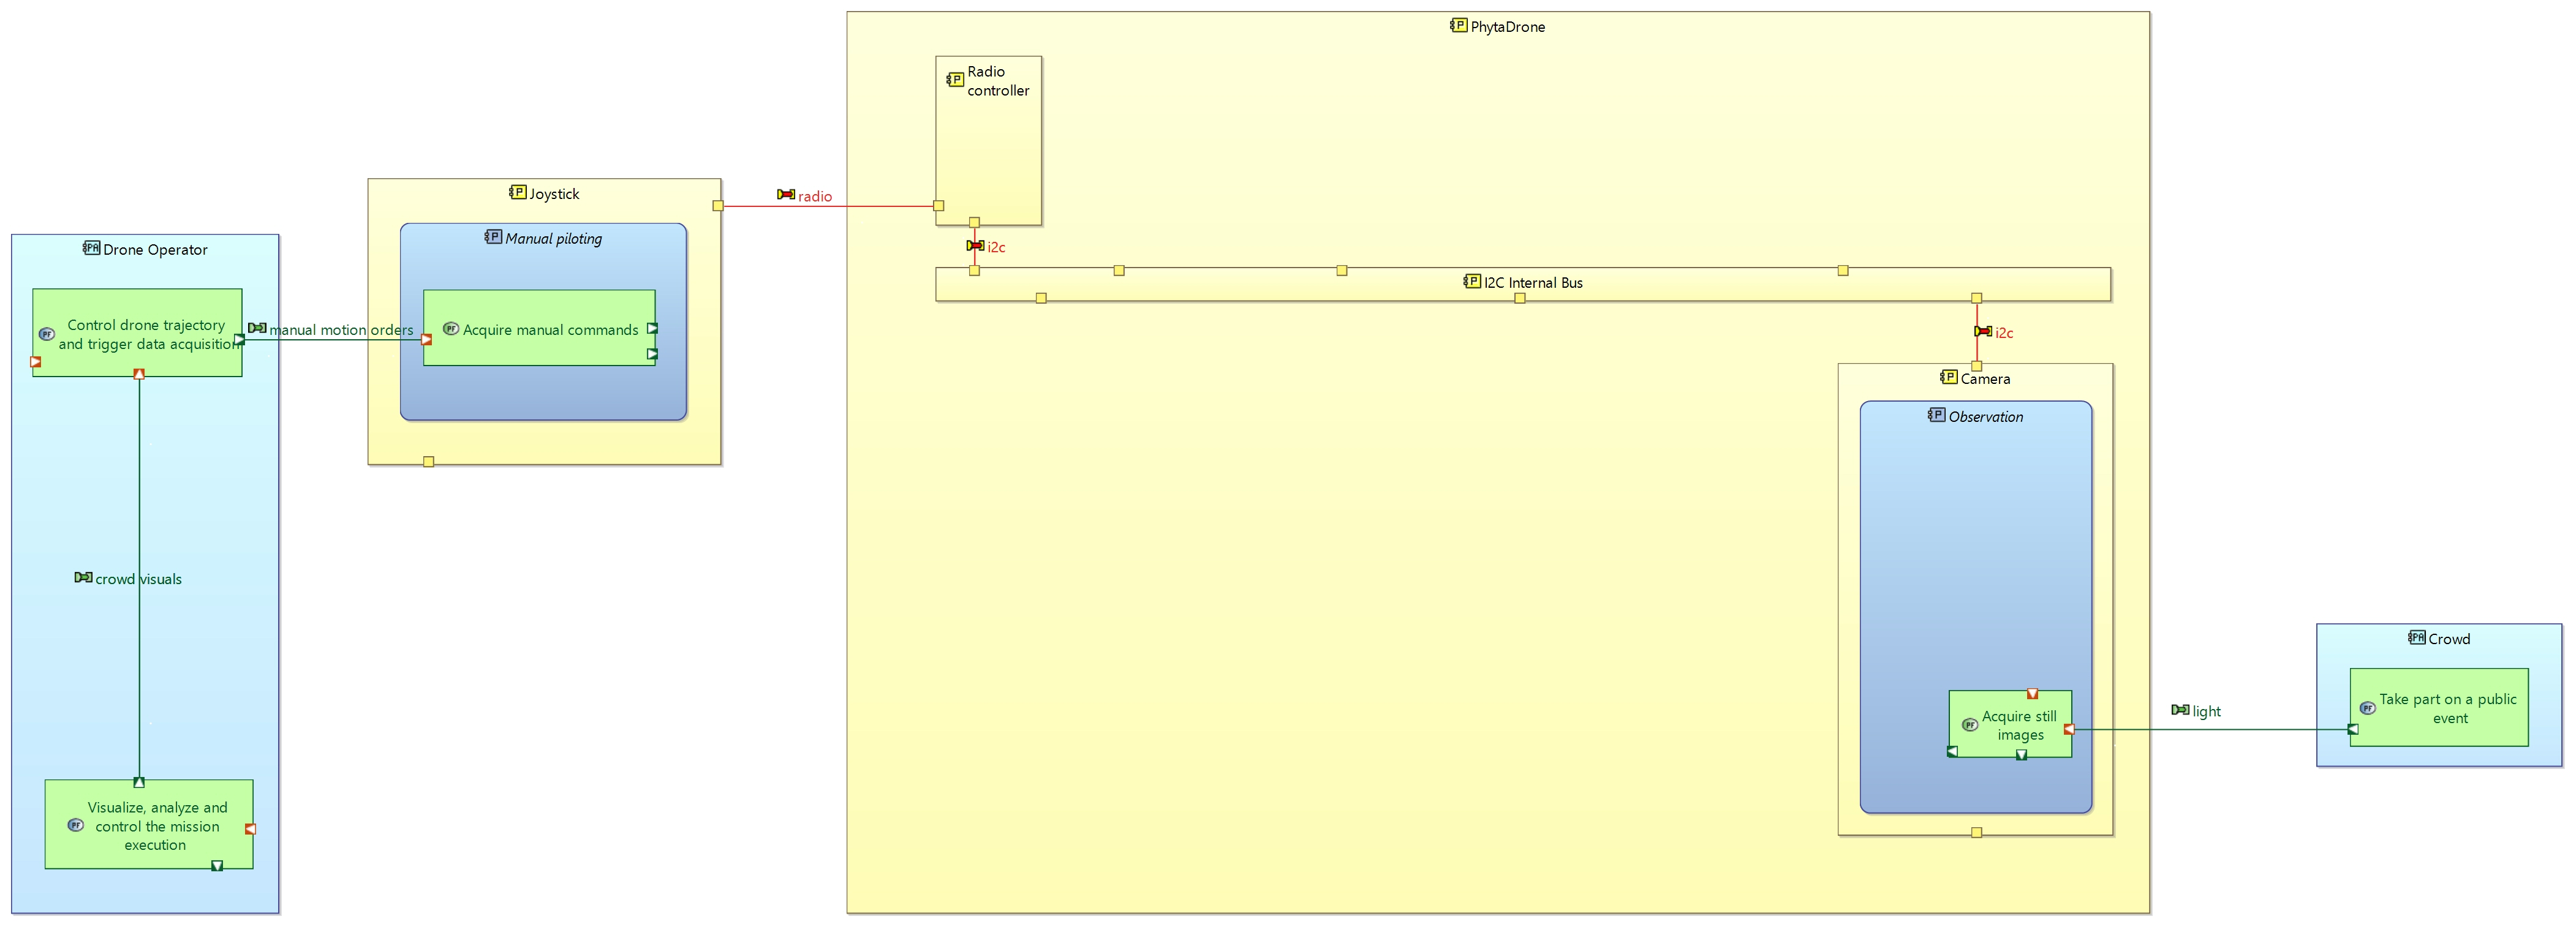
\includegraphics[width=\textwidth, height=6.75cm, keepaspectratio]{./images/EX2/CSC_5RO08_TA_EX2_PAB_Low.jpg}
            % \caption{}
        \end{figure}
    \end{frame}


    \section*{Q\&A}

    \maketitle

\end{document}